\documentclass[runningheads,a4paper]{llncs}
\usepackage[utf8]{inputenc}
\usepackage{amsmath}
\usepackage{amssymb}
\usepackage{enumerate}
\usepackage{xspace}
\usepackage{graphicx}
\usepackage{subcaption}
\usepackage{hyperref}
\usepackage{xypic}

%\title{Grid USO algorithms}
%\author{Antonis Thomas \\ \small ETH Zürich \and
   %     Jerri Nummenpalo \\ \small ETH Zürich \and
   %     Luis Barba \\ \small ULB / Carleton University \and
   %     Malte Milatz \\ \small ETH Zürich}

\newtheorem{observation}{Observation}
%\newtheorem{lemma}{Lemma}
%\newtheorem{definition}{Definition}
%\newtheorem{corollary}{Corollary}
%\newtheorem{theorem}{Theorem}
%\newtheorem{prop}{Proposition}
%\newtheorem{conjecture}{Conjecture}

%%%%%%%%%%%%%%%%%%%%%%%%%%%%%%%%%%%%%%%%%%%%%%%%%%%%%%%%%%%%%%%%%%%%%%
% Setup margin comments. If you want to ignore them, then comment the other part out.
\newcommand{\JN}[1]{\marginpar{\parbox{4cm}{{\small {\bf JN:} #1}}}} %Jerri
\newcommand{\LB}[1]{\marginpar{\parbox{4cm}{{\small {\bf LB:} #1}}}} %Luis
\newcommand{\MM}[1]{\marginpar{\parbox{4cm}{{\small {\bf MM:} #1}}}} %Malte
\newcommand{\AT}[1]{\marginpar{\parbox{4cm}{{\small {\bf AT:} #1}}}} %Antonis
\newcommand{\BG}[1]{\marginpar{\parbox{4cm}{{\small {\bf BG:} #1}}}} %Bernd
%\newcommand{\JN}[1]{}

%%%%%%%%%%%%%%%%%%%%%%%%%%%%%%%%%%%%%%%%%%%%%%%%%%%%%%%%%%%%%%%%%%%%%%

\newcommand{\indegree}{refined in-degree\xspace}
\newcommand{\ind}{\ensuremath{\mathrm{ind}}}
\newcommand{\og}{\overrightarrow{G}}
\newcommand{\A}{\ensuremath{\mathcal A}}
\newcommand{\B}{\ensuremath{\mathcal B}}
\newcommand{\s}[1]{\ensuremath{s_{\scriptscriptstyle#1}}}
\newcommand{\USO}{\ensuremath{\mathrm{USO}}}
\newcommand{\timeEdge}{\ensuremath{T_\mathrm{E}}}
\newcommand{\timeVertex}{\ensuremath{T_\mathrm{V}}}
\newcommand{\e}{\ensuremath{\mathrm{e}}}
\newcommand{\RR}{\ensuremath{\mathbb{R}}}
\newcommand{\Sym}{\ensuremath{\mathfrak{S}}}
\newcommand{\Tr}{\ensuremath{\mathrm{Tr}}}
\newcommand{\sink}{\ensuremath{\mathrm{sink}}}
\newcommand{\join}{\mbox{join}\xspace}

\begin{document}

\mainmatter  % start of an individual contribution

% first the title is needed
\title{Algorithms for Grid Unique sink orientations}

% a short form should be given in case it is too long for the running head
%\titlerunning{}

% the name(s) of the author(s) follow(s) next
%
% NB: Chinese authors should write their first names(s) in front of
% their surnames. This ensures that the names appear correctly in
% the running heads and the author index.
%
\author{Luis Barba\thanks{Possible thanks to someone.}\inst{1} \and Malte Milatz\inst{2} \and Jerri Nummenpalo\inst{2} \and Antonis Thomas\inst{2}}%

%
\authorrunning{Grid USO algorithms}
% (feature abused for this document to repeat the title also on left hand pages)

% the affiliations are given next; don't give your e-mail address
% unless you accept that it will be published
\institute{Luis' affiliations \url{possible_url} 
\and
ETH Z{\"u}rich, Department of Computer Science \\
CH-8092 Z{\"u}rich, Switzerland
}

%
% NB: a more complex sample for affiliations and the mapping to the
% corresponding authors can be found in the file "llncs.dem"
% (search for the string "\mainmatter" where a contribution starts).
% "llncs.dem" accompanies the document class "llncs.cls".
%

%\toctitle{Lecture Notes in Computer Science}
%\tocauthor{Authors' Instructions}
\maketitle

\begin{abstract}
\noindent
    We study unique sink orientations (USOs) of \emph{grids}, which for us are
    Cartesian products of two complete graphs.
    We show that the sink in a grid USO can be found deterministically using
    $O(N \log N)$ vertex queries, or using $O(N^{\log_4 7})$ edge queries.
    On the other hand we argue that a linear number of queries is necessary.
    Furthermore we analyze the number of grid USOs.
    \keywords{Unique sink orientation}
\end{abstract}

\section{Introduction}

\subsection{[Summary of who has done what when it comes to grid USOs]}

In the text below grid means 2-dimensional unless explicitly mentioned otherwise.

In \cite{linepointstoc} we find the first reference to grid USOs. The concrete problem they solve is ``One line and $n$ points''. The input is $n$ points in general position and one vertical line which is disjoint from the points and all intersections of segments connecting pairs of points. The problem is to find the lower most segment connecting a pair of points (one point in each side of the line). This appears to be\AT{Luis will know more here.} a common subprocess of geometric algorithms.  (Note that \cite{linepointstoc} talks about unique sink orientations of grid -even though it does not coin the term- and is a few months before \cite{SW}). They prove that every instance of one line and $n$ points gives rise to a grid USO. In addition, they design an instance of a grid USO that does not come from a one line and $n$ points instance\AT{They also show pseudorealizability but maybe we don't even want to mention that, i.e. look at section 5 of \cite{linepointstoc}}. They give a randomized algorithm (which is essentially equivalent to Random Edge) for one line and $n$ points which runs in $O(\log^2 n )$ pivot steps. They also give an instance where the algorithm needs $\Omega(\log^2 n )$ many pivot steps. 

In \cite{linepoint} and \cite{falkthesis} they argue that the proofs discussed in \cite{linepointstoc}, mentioned in the previous paragraph, can be translated to the more general grid USO setting. So far all the results have been about \emph{admissible} grid orientations. Those are unique sink, acyclic and have a forbidden minor; there is no subgrid isomorphic to a specific (3,2)-grid that later was called ``double twist''.

In \cite{grid05} they go further and prove that every admissible grid orientation is induced by a red-bue arrangement of pseudolines (this needs to be discussed further). Moreover, they define the refined index and they prove that the refined index of every grid USO is a bijection. They show that the a grid USO is Holt-Klee if and only if it does not have an induced double twist. In addition, they generalize the result of \cite{linepoint} to conclude that Random Edge needs at most $O(\log(n+1)\log(m+1))$ pivot steps to find the sink of any Holt-Klee grid USO and any starting vertex. Finally, they argue that there is at least $2^{\Omega(n^2)}$ different admissible (Holt-Klee) (n,m)-grid USO.

In \cite{grid08}, they study large dimension grid USO as general models that arise from solving PGLCP (to be defined?). They give a randomized product algorithm (similar in spirit to the one introduced in \cite{SW} for cube USO) and prove that for fixed dimension it runs in polylogarithmic time. Namely, for the 2-dimensional case it runs in time $O(\ln^2 n)$, thus matching the upper bound for admissible grid orientations. Finally, they prove that any grid USO is acyclic.

Note that the complexity of Random Edge on general grid USO remains open.

\subsection{[Short Motivation]}

Unique sink orientations of grids, as introduced in \cite{linepointstoc},
are a graph-theoretic model for a specific class of linear programs.
Namely, assume that the feasible region of a given linear program is a
simple polytope of dimension $d$ that has exactly $d+2$ facets.
The graph $G$ underlying such a polytope is isomorphic to a Cartesian product
of two complete graphs, $G = K_m \times K_n$.
(A proof of this theorem can be found in \cite{grid05}.)

Let $f : \RR^d \to \RR$ denote the objective function of the linear program.
Assuming general position, one can orient $G$ such that for every oriented
edge $u \to v$ we have $f(u) > f(v)$.
Minimizing the function $f$ on the polytope thus corresponds to finding the
unique sink of $G$.

\subsection{Summary of Results}

Given a unique sink orientation of the grid $G = K_m \times K_n$, the
algorithmic task is to find its sink.
We consider two different settings:
\begin{enumerate}[\quad (1)]
    \item
        The algorithm accesses the grid $G$ by means of an \emph{edge oracle}
        which, when queried about an edge of $G$, reveals its orientation.
        The goal of the algorithm is to report the sink of $G$.

    \item
        The algorithm accesses the grid $G$ by means of a \emph{vertex oracle}
        which, when queried about a vertex of $G$, reveals the orientations of
        the edges adjacent to this vertex.
        The goal of the algorithm is to query the sink of $G$.

\end{enumerate}
For both problems we restrict our attention to deterministic algorithms, and
we pursue the following question:
\begin{quote}
    Among all deterministic algorithms for problem (1) or (2), respectively,
    what is the minimum number of queries that the algorithm must ask in the
    worst case?
\end{quote}
We will denote this number by $\timeEdge(N)$ and
$\timeVertex(N)$, respectively, where $N := m + n$.
Our results are:

\begin{itemize}
    \item
        $\timeVertex(N) \in O(N \log N)$ (Theorem~\ref{theorem:Sink algorithm}).
    \item
        $\timeVertex(N) \ge N-1$ (Theorem~\ref{thm:lowerbound}), and this
        inequality becomes an equality when $m = n \le 4$
        (theorem \ref{thm:smallGrids}).
    \item
        $\timeEdge(N) \in O(N ^ { \log_4(7) })$ (Theorem~\ref{thm:timeEdge}),
        and $\timeEdge(N) \in \Omega(N)$.
\end{itemize}
We also show that the number of unique sink orientations of $K_n \times K_n$
is $\e^{ \Theta(n^2 \log n) }$ (Theorem~\ref{thm:asymptotics-USO-nn}).

\subsection{Outline}

The rest of this paper is organized as follows.
We start by defining terminology and basic properties of grids in Section \ref{section:grid_uso_properties}.
Section \ref{section:The vertex oracle model} assumes the vertex oracle model;
it contains our main result (Theorem~\ref{theorem:Sink algorithm})
as well as our lower bound.
Section \ref{section:The edge oracle model}, on the other hand, assumes the
edge oracle model.
In Section \ref{section:counting_unique_sink_orientations} we count the number of unique sink orientations.

\section{Grid USO Properties}
\label{section:grid_uso_properties}

\subsection{Grids, Subgrids and Orientations}

We write $K_X$ for the complete graph on a given vertex set $X$.
Given two finite sets $X$ and $Y$,
the \emph{$X \times Y$-grid} is the product graph $G = K_X \times K_Y$.
It is also called an \emph{$(m,n)$-grid}, where $m = |X|$ and $n = |Y|$ denote
the cardinalities of the index sets.
Unless otherwise specified, we assume that $X = [m]$ and $Y = [n]$.
See Figure~\ref{fig:examplegrid} for an example of a grid.

Explicitly, the vertex set of the graph $G$ is $X \times Y$, and two
vertices $v,w \in X \times Y$ are adjacent if and only if they differ in
exactly one of the two coordinates.
We call the edge $vw$ a \emph{horizontal edge} if $v$ and $w$ differ in the
$X$-coordinate, and we speak of a \emph{vertical edge} if they differ in the
$Y$-coordinate. The \emph{rows} and \emph{columns} of the grid are defined accordingly.

An induced subgraph of a grid is called a \emph{subgrid} if it is itself a grid.
The subgrids of $G$ are exactly those induced subgraphs whose vertex set is a
Cartesian product $I \times J$, for some $I \subseteq X$ and $J \subseteq Y$.
If the graph $G$ is oriented then its subgrids inherit an orientation.

  \begin{figure}[htbp] 
  	\centering
  	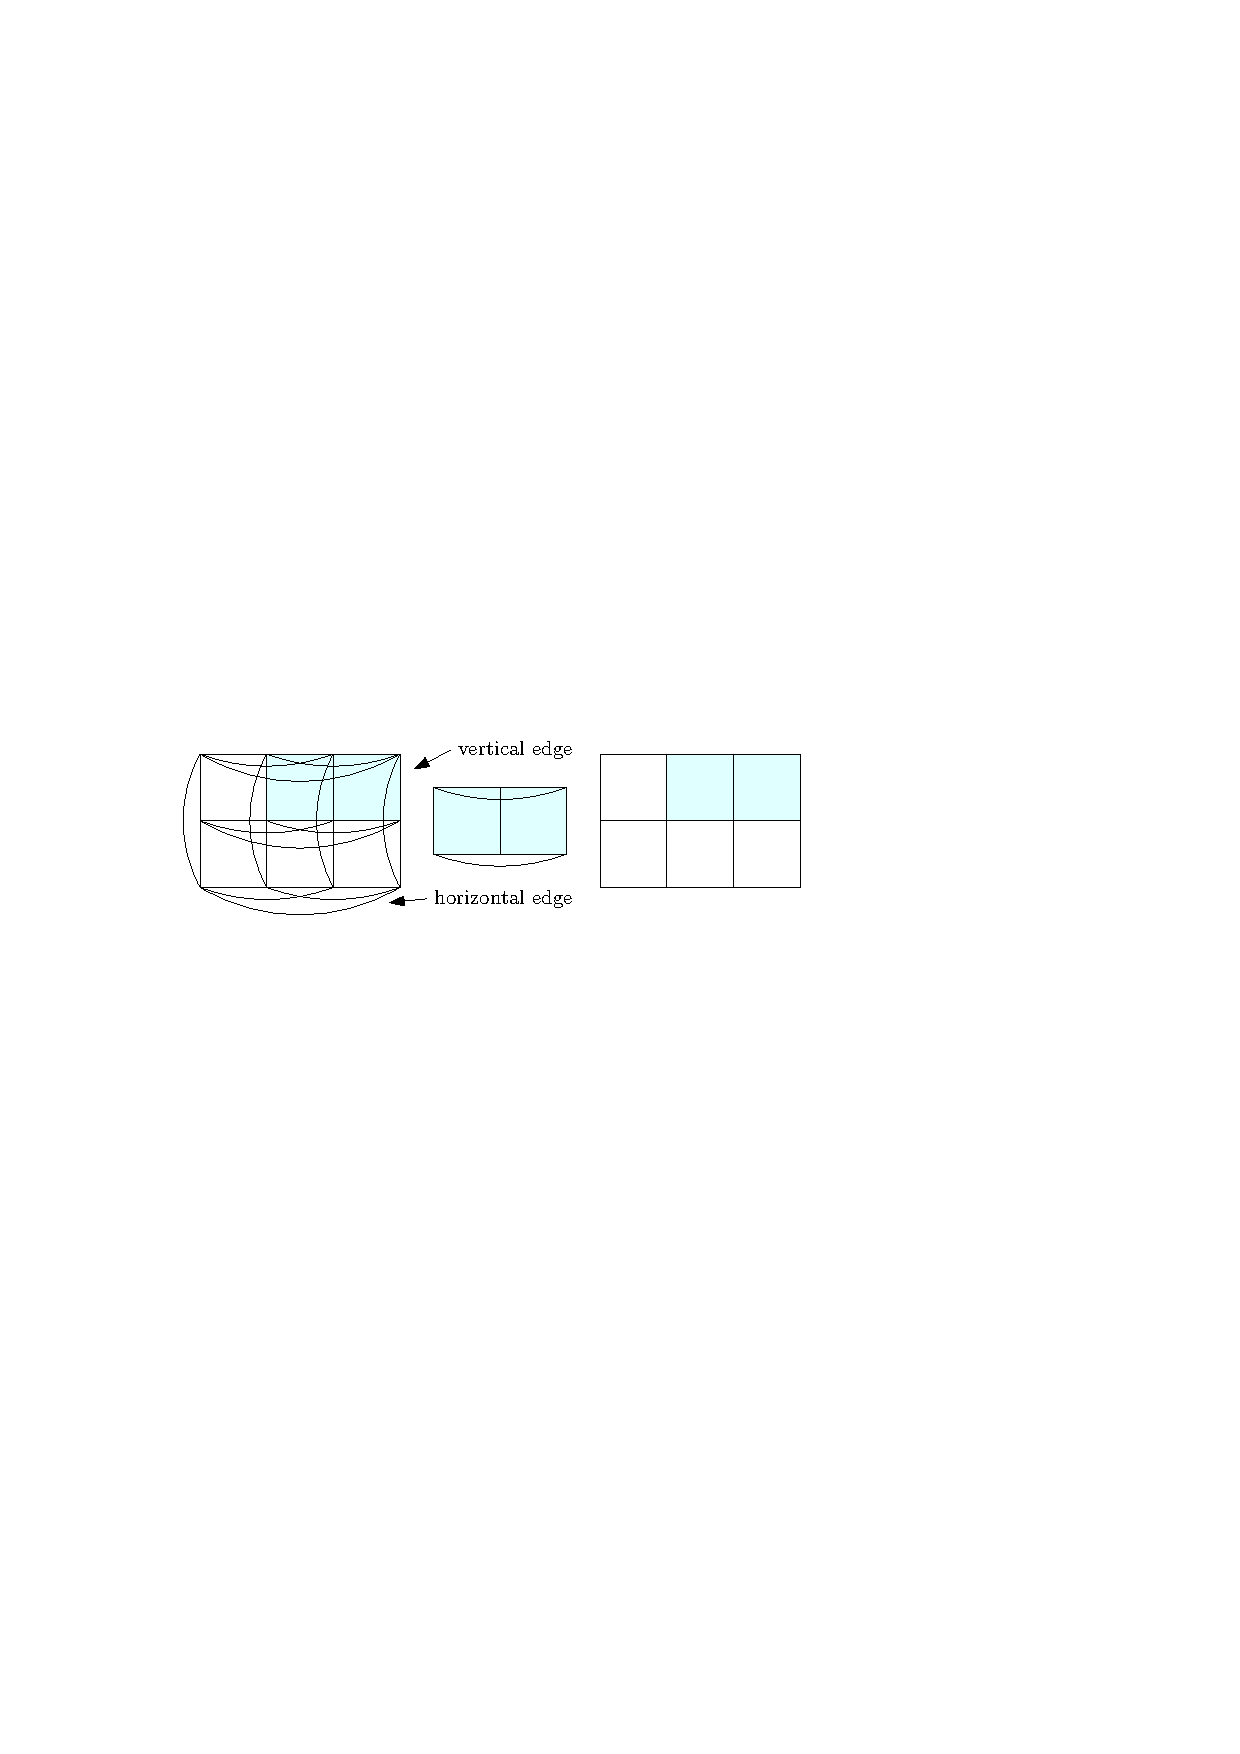
\includegraphics[scale=1.0]{uso_example.pdf}
  	\caption{\small On the left an exampe of an (4,3)-grid. A $(3,2)$-subgrid is higlighted in color and displayed separately in the middle. In the subsequent figures we will not draw all the edges, but rather as in the grid displayed on the right where some edges have been omitted. The definition of horizontal and vertical edges is also being displayed.} 
  	\label{fig:examplegrid}
  \end{figure}

A vertex in an oriented graph is called a \emph{sink} if all its incident edges are incoming.
An orientation of a grid is a \emph{unique sink orientation}, or \emph{USO}
for short, if all its non-empty subgrids have a unique sink. For simplicity, we call a grid with a unique sink orientation a grid USO.



%\begin{lemma}[Product construction]
% Let $G$ be an $X\times Y$-grid USO for some sets $X$ and $Y$ and let $A \subset 2^X$ and $B \subset 2^Y$ be partitions of $X$ and $Y$, respectively. Let $H$ be an $A\times B$-grid. \JN{See Malte's 4$\times$4 lower bound for a possible way to define this.}
%\end{lemma}

\subsection{Basic Properties}

We will start by stating certain basic properties of grid USOs.

\begin{lemma}[\cite{grid08}]
\label{lemma:acyclicity_lemma}
 Grid unique sink orientations are acyclic.
\end{lemma}

A useful property of grids is that one can test whether an orientation is a unique sink orientation by only looking at small subgrids as stated by the next proposition.

\begin{proposition}
\label{prop:subgrid_uso_check}
 An orientation of a grid is a unique sink orientation if and only if it is acyclic and every $(2, 2)$-subgrid is a unique sink orientation.
\end{proposition}

\begin{proof}
 One direction is evident: If a grid orientation is a unique sink orientation, then every $(2,2)$-subgrid is also a unique sink orientation and by Lemma~\ref{lemma:acyclicity_lemma} the orientation is acyclic. 
 For the other direction note that every $(1,k)$-subgrid and $(k,1)$-subgrid is a unique sink orientation due to acyclicity. 
 If there were two sinks in any other subgrid, then we could find a $(2,2)$-subgrid that was not a unique sink orientation which would contradict the assumption.
 Acyclicity proves the existence of one sink in each subgrid and the statement follows. \qed
\end{proof}

\subsection{Induced USOs}

When designing algorithms for grids, at some point one will typically want to
partition the grid into subgrid.
Such a partition into subgrids forms itself a grid in a natural way,
and we define a unique sink orientation on the induced grid.
To distinguish between the original grid and the induced grid, we refer to the vertices of the induced grid as blocks.
An example of an induced unique sink orientation is shown in Figure~\ref{fig:example_induced_orientation}.

  \begin{figure}[htbp] 
  	\centering
  	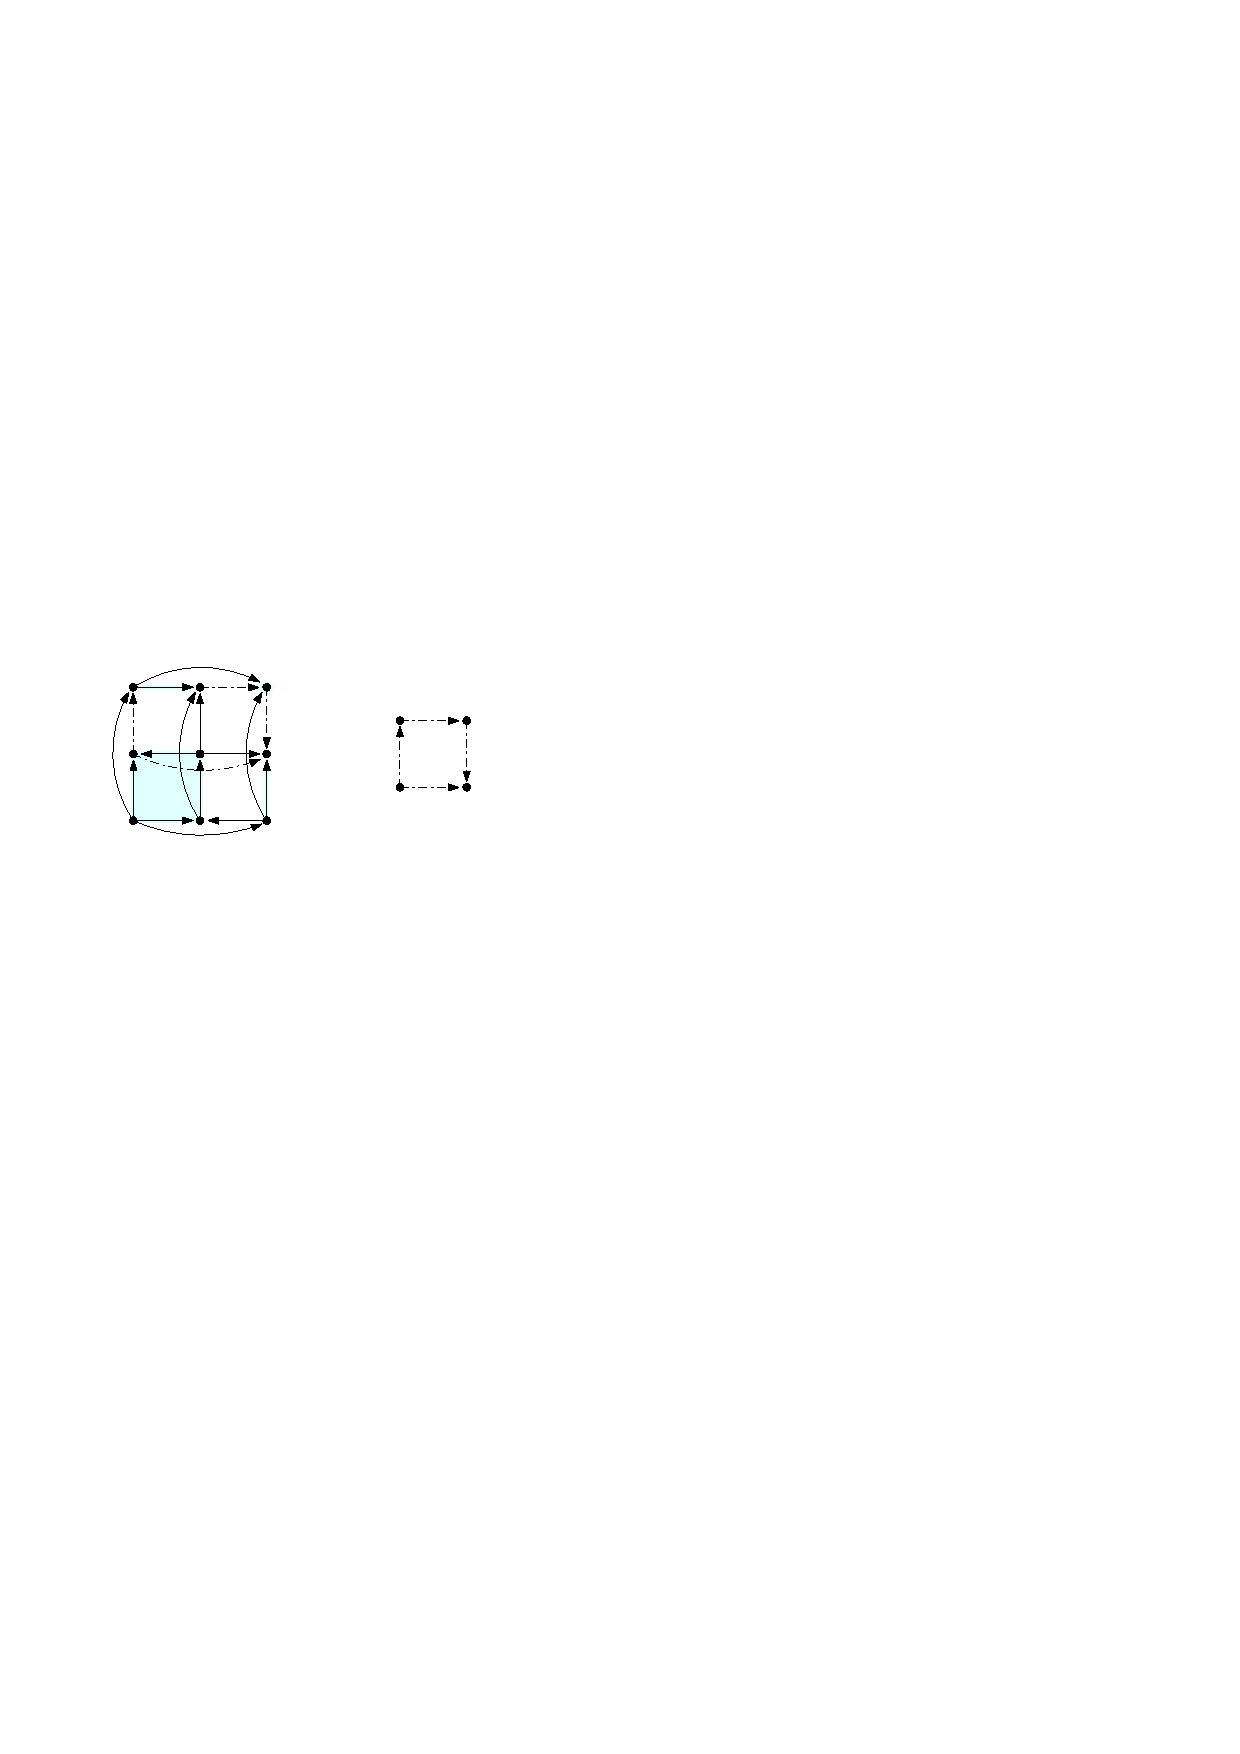
\includegraphics[scale=1.5]{induced_orientation_ex.pdf}
  	\caption{\small On the left side of the figure there is a $(3,3)$-grid USO whose $X$-coordinates and $Y$-coordinates have been partitioned into 2 parts of cardinalities two and one. This induces four blocks as highlighted in bold and blue. The induced orientation with respect to these blocks is shown on the right and the edges contributing are also shown in the original grid.} 
  	\label{fig:example_induced_orientation}
  \end{figure}

Formally, let $G = K_X \times K_Y$ be a grid USO,
and let $\A$ and $\B$ be partitions of $X$ and $Y$, respectively.
Let $H = K_\A \times K_\B$ be the \emph{$\A$-$\B$-partition grid} of $G$.
For every vertex $x = (A,B)$ of $H$, where $A\in \A$ and $B \in \B$, let $G(x)$ (or simply $G(A,B)$)
denote the $A \times B$-subgrid of $G$. 
The edge between two adjacent vertices $x$ and $y$ of $H$ is oriented towards $y$ if the sink of $G(x)$ has at least one outgoing edge to a vertex of $G(y)$ in the original grid $G$. 
This orientation is well defined, because if the sink of $G(y)$ had an edge towards some vertex of $G(x)$, there would be a cycle in $G$. 
Furthermore, there is always at least one such outgoing edge from one of the sinks as otherwise an appropriately chosen subgrid of $G$ would have two sinks. 
We say that is orientation is \emph{induced} on $H$ by $G$.

\begin{lemma}[USO-Lemma]\label{lemma:USO-Lemma}
Let $G = K_X \times K_Y$ be a grid unique sink orientation,
and let $\A$ and $\B$ be partitions of $X$ and $Y$, respectively.
The orientation of the $\A$-$\B$-partition grid $H = K_\A \times K_\B$ induced by $G$ is a unique sink orientation.
\end{lemma}

\begin{proof}
Let $A, A'\in \A$ and $B,B'\in \B$. Let $F$ be the $\{A,A'\}\times\{B, B'\}$-subgrid of~$H$.
Note that $F$ consists of four blocks being $(A,B), (A', B), (A, B')$ and $(A', B')$. Let their respective sinks be $s_{A,B}$,$s_{A',B}$,$s_{A,B'}$ and $s_{A',B'}$.
By Proposition \ref{prop:subgrid_uso_check} it is enough to check that the orientation of $F$ is a unique sink orientation and that $H$ is acyclic.
We first show that $F$ has at most one sink and then show that it cannot have cycles and therefore has exactly one sink. Lastly we show that $H$ can not have cycles.

Assume for a contradiction that $F$ has more than one sink.
Because these sinks cannot be adjacent, $F$ has two sinks and without loss of generality they are the blocks $(A,B')$ and $(A', B)$. Consider the $(2,2)$ subgrid in $G$ that contains the vertices $\s{A,B'}$ and $\s{A',B}$. By assumption, and from the way the induced orientation was constructed, this subgrid has two sinks which is a contradiction to $G$ being a unique sink orientation. See Figure~\ref{fig:InducedUSOtwosinks} for an example. Therefore we conclude that $F$ has at most one sink. 

Next to show is that $F$ has at least one sink. The only way for $F$ to have no sink is if there is a cycle in $F$. Such a cycle would induce a cycle in $G$: starting from the sink of one of the blocks of $H$, move along an edge to another block and then again to the sink of the new block and repeat until we reach the sink of the block we started from. This works because there is always such an outgoing edge between blocks when $F$ is cyclic --- which implies an outgoing edge in the original grid --- and there is always a path within a block from any vertex to the sink of the block due to Lemma~\ref{lemma:acyclicity_lemma}. Such a cycle is illustrated in Figure~\ref{fig:InducedUSOcycle}. We conclude that $F$ can't have a cycle and therefore $F$ will have exactly one sink.

To see that $H$ is acyclic one only needs to repeat the same argument as for $F$. That is, a cycle in $H$ would imply a cycle in $G$. This concludes the proof. \qed

\begin{figure}
\begin{subfigure}[t]{0.45\textwidth}
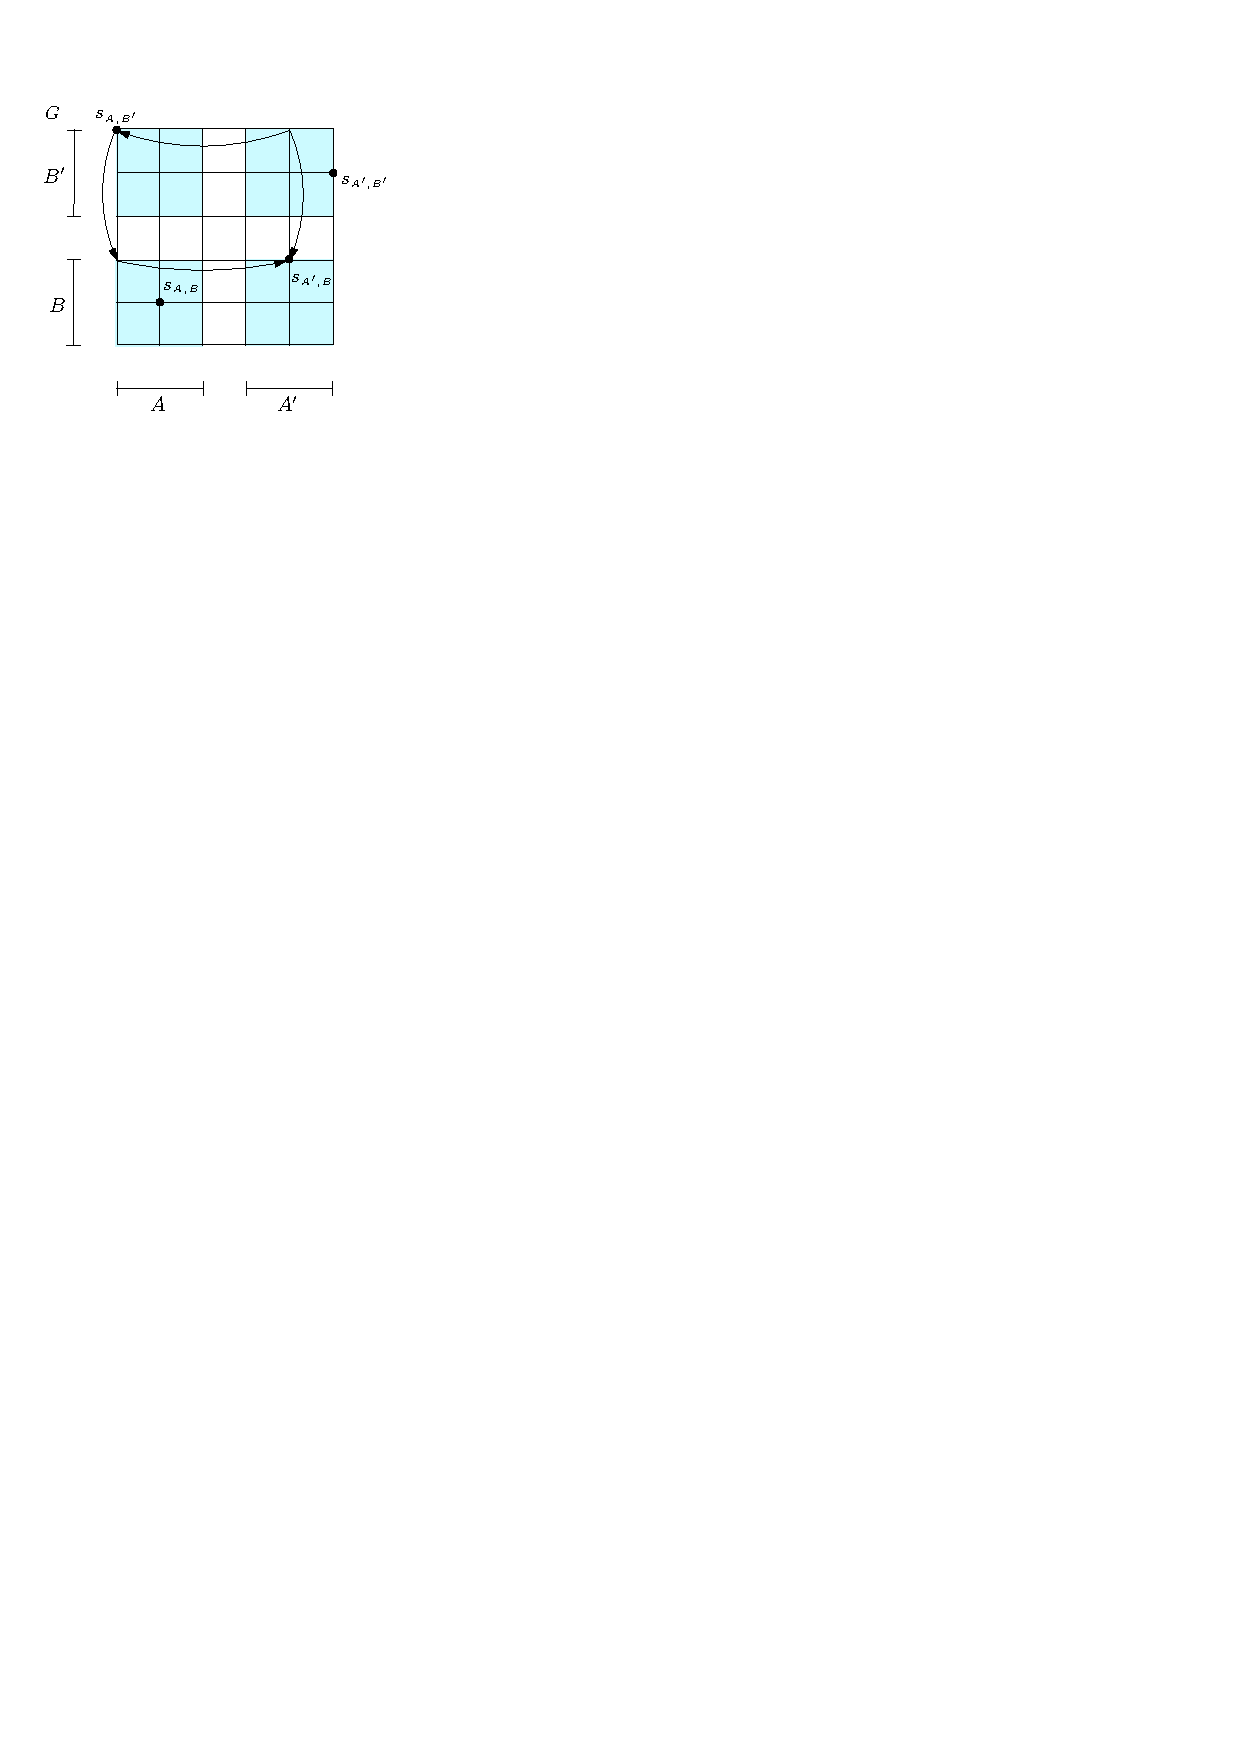
\includegraphics{product_lemma_two_sinks.pdf}
%[width=1\textwidth]
\caption{\small If the induced grid USO F had two sinks, a (2,2) grid in the original grid $G$ wouldn't have a unique sink.}
\label{fig:InducedUSOtwosinks}
\end{subfigure}
\qquad\qquad
\begin{subfigure}[t]{0.45\textwidth}
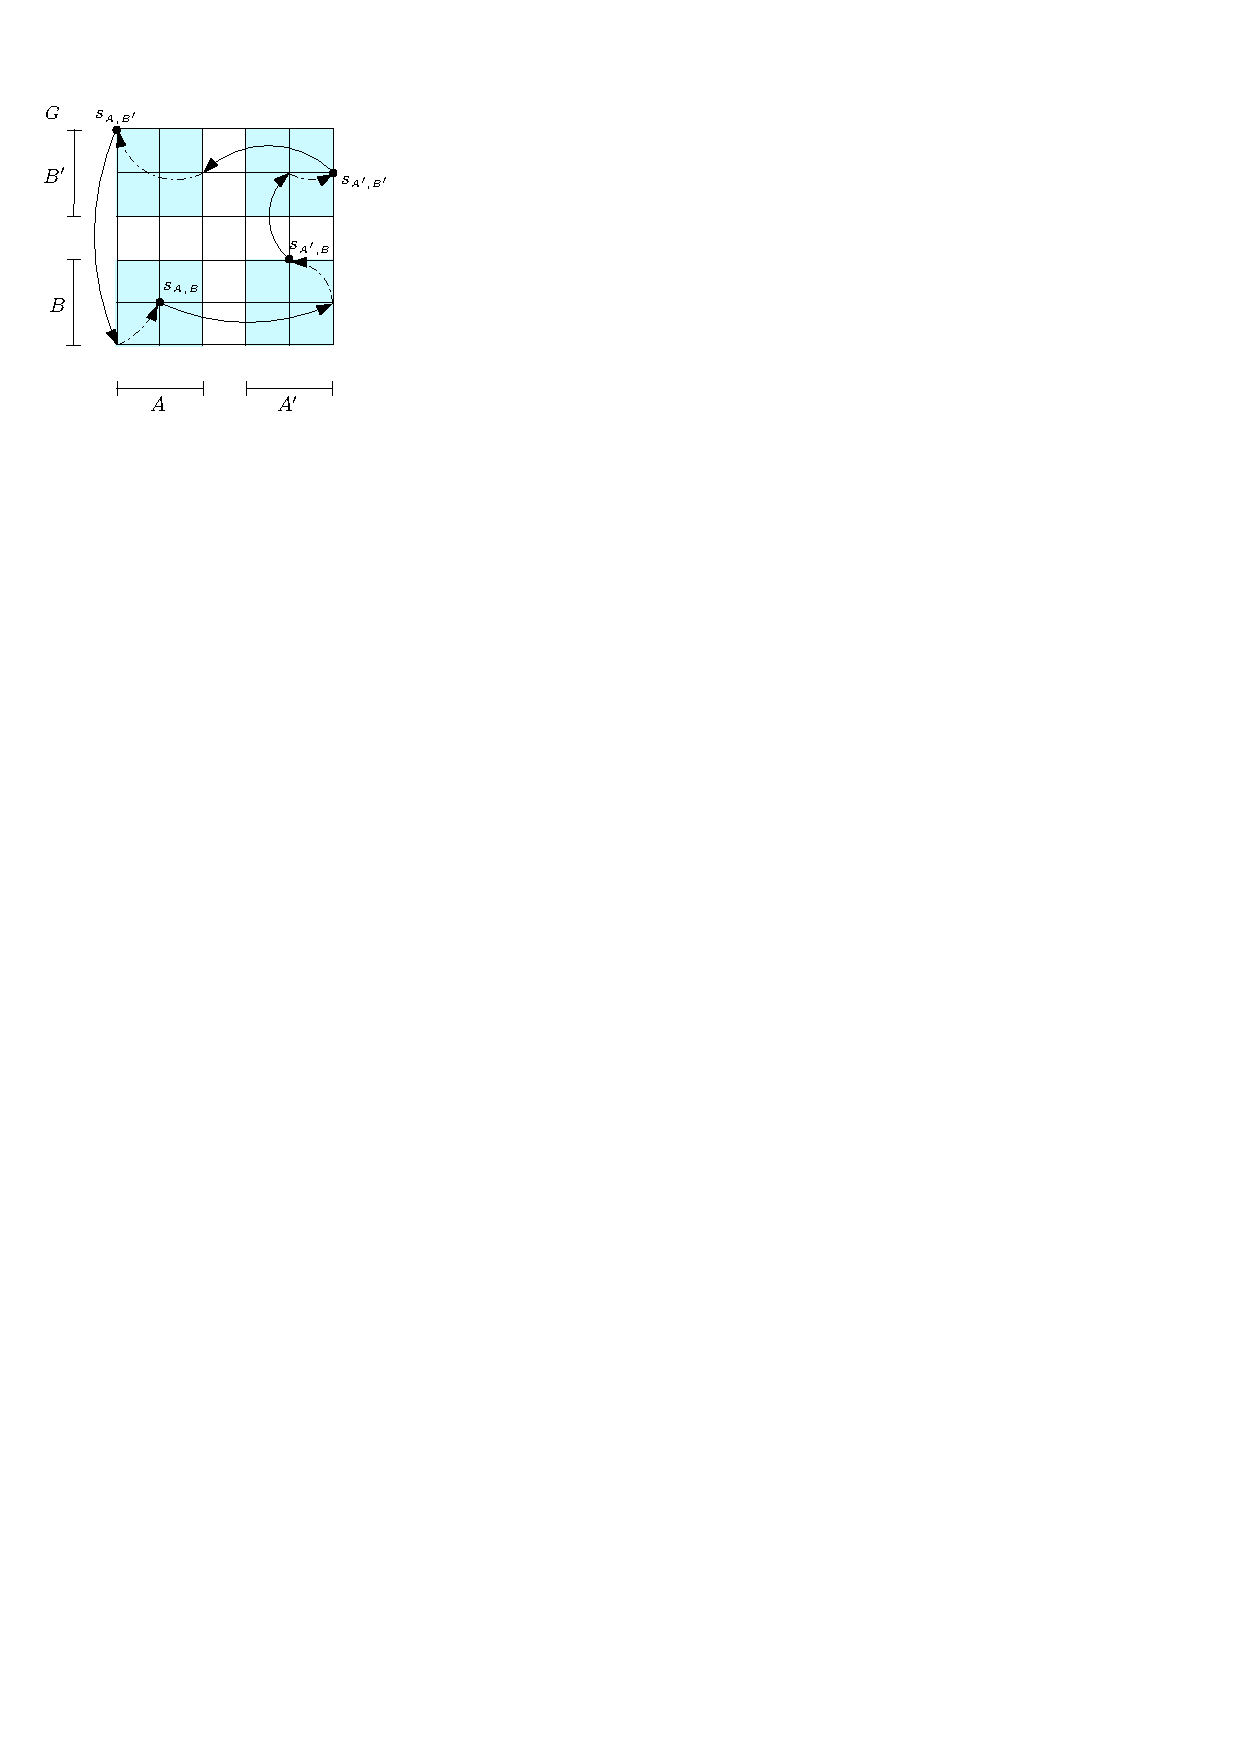
\includegraphics{product_lemma_cycle.pdf}
\caption{\small If the induced USO F had a cycle, there would be a cycle in the original grid $G$.}
\label{fig:InducedUSOcycle}
\end{subfigure}
\caption{An illustration of the two cases in the proof of Lemma~\ref{lemma:USO-Lemma}. Solid arrowed edges represent edges in $G$ and dashed edges represent (directed) paths in $G$.}
\label{fig:inducesUSOboth}
\end{figure}

\end{proof}

\begin{theorem}
\label{thm:the_sink_of_the_sink_of_the_induced_orientation_is_the_global_sink}

Let $G = K_X \times K_Y$ be an oriented grid,
and let $\A$ and $\B$ be partitions of $X$ and $Y$, respectively.
If $(A,B)$ is the sink of the $\A$-$\B$-partition grid $H = K_\A \times K_\B$, then the sink of $G(A,B)$ is the sink of $G$.
\end{theorem}
\begin{proof}
Let $\s{A,B}$ be the sink of $G(A,B)$ and let $\s{G}$ denote the sink of $G$.
We claim that $\s{G} = \s{A,B}$.
Assume for a contradiction that $\s{A,B}\neq \s{G}$.
Note that $\s{G}$ does not belong to $G(A,B)$ as $\s{A,B}$ is its sink.
Therefore, $\s{G}$ is the sink of $G(A', B')$ for some $A'\in \A, B'\in \B$.

Consider the smallest subgrid in $H$ containing both $(A,B)$ and $(A', B')$. 
Since Lemma~\ref{lemma:USO-Lemma} guarantees that $(A',B')$ is not the sink of this subgrid, there is at least one outgoing edge from $(A',B')$ to another vertex.
Thus, by the definition of the orientation of $H$, there is an outgoing edge going from the sink of $G(A',B')$, i.e., an outgoing edge from $\s{G}$---a contradiction since $\s{G}$ is the sink of $G$ and has no outgoing edges. 
Therefore, $\s{G} = \s{A,B}$. \qed
\end{proof}


\section{The Vertex Oracle Model}
\label{section:The vertex oracle model}

\subsection{The Sink-finding Algorithm}
\label{section:the_sink_finding_algorithm}

Before explaining the algorithm we introduce some notation. We define a partial order of vertices in a grid unique sink orientation $G$ as follows. 
For any two vertices $v,w \in G$ we say that $w \succeq v$ if there is a directed path from $w$ to $v$ within the grid $G$. In words, we say that $w$ is \emph{larger} than $v$ (or $v$ is \emph{smaller} than $w$).
Because by Lemma~\ref{lemma:acyclicity_lemma} grid USOs are acyclic, this partial order is well defined.
The sink of the grid USO is the unique minimal vertex with respect to this ordering. For $v,w \in G$ we also define an operation called \emph{\join} so that \join($v,w$) is the vertex that is the sink in the smallest subcube containing $v$ and $w$. Note that $v,w \succeq \join(v,w)$. For sets of vertices $V$, $\join(V)$ denotes the set of vertices of the grid to which there is a path from all vertices in $V$. More formally $\join(V) = \{w \in G \: | \: v \succeq w \:\: \forall v \in V \}$. Given some set of vertices $V$ we can compute some $w \in \join(V)$ with $\mathcal{O}(|V|)$ vertex queries: just repeatedly apply the $\join$ operation on vertices from $V$.

%Note that two vertices may not be $\succeq$-comparable in the smallest subgrid containing them. 
%There could still be a path between the two vertices. 
%Thus\JN{after the transitive closure they might still be incomparable}, we consider the transitive closure of this relation and say that a vertex $w$ is \emph{larger} than $v$ (or $v$ is smaller than $w$) if there is a sequence $w = v_1, v_2, \ldots, v_k = v$ of $G$ such that $v_i \succeq v_{i+1}$, for each $1\leq i\leq k-1$.

In an ($m,n$)-grid USO $G$, the \emph{\indegree} of a vertex $v \in G$ is an ordered pair $[a_v, b_v] \in \{0,1,\ldots,m-1\}\times \{0,1,\ldots,n-1\}$ where $a_v$ and $b_v$ specify the number of incoming horizontal  and vertical edges of $v$, respectively.
We say that a vertex $v$ with \indegree $[a_v, b_v]$ is a \emph{$(k, t)$-vertex} if $a_v\geq k-1$ while $b_v\geq t-1$.

Consider the following algorithmic approach to finding the sink of an ($n$,$n$)-grid USO deterministically. 
Assume that we are able to find in $\mathcal{O}(n)$ time a $(\frac{n}{2}, \frac{n}{2})$-vertex $v$.
We could then partition the grid into 4 equally sized square subgrids so that $v$ is the sink of one of the subgrids.
The next step would be to find the sink of the subgrid opposite to the partition containing $v$ in the induced (2,2)-grid. 
By Theorem~\ref{thm:the_sink_of_the_sink_of_the_induced_orientation_is_the_global_sink} we could thereafter discard one subgrid out of consideration and possibly still find the sink of one subgrid.
If one finds the sinks of the subgrids recursively, one would get the recursion
\begin{align*}
 T(n) = 2T\left(\frac{n}{2}\right) + \mathcal{O}(n)
\end{align*}
where $T(n)$ is the number of vertex queries needed to find the sink of an $(n,n)$-grid. By the master theorem we would have that $T(n) = \mathcal{O}(n\log n)$. 
As a first step, we show how to compute an $(\frac{n}{4}, \frac{n}{4})$-vertex of an $(n, n)$-grid. Then, we extend this result to non-square grids. Finally, using these results as a black box, we show how to compute an $(\frac{m}{2}, \frac{n}{2})$-vertex in an $(m,n)$-grid using $O(n+m)$ vertex queries in total and then conclude with our main result in Theorem~\ref{theorem:Sink algorithm}. 

\begin{lemma}
\label{lem:seed_lemma_for_square_matrices}
 Given an $[n]\times [n]$ grid USO we can find an $(\frac{n}{4}, \frac{n}{4})$-vertex using $\mathcal{O}(n)$ vertex queries.
\end{lemma}

\begin{proof}
The algorithm we describe queries a linear number of vertices of the grid before finding a vertex with the required \indegree. 
After explaining the algorithm we prove its correctness.
  
The algorithm works as follows. First, query the diagonal vertices $D = \{v_1,\ldots, v_n\}$ where $v_i = (i,i)$. textnormal
If one of the vertices in $D$ has the required \indegree, we are done. 
If not, observe that we can assume (by sorting and renaming) that vertex $v_i$ has at least $i-1$ incoming edges. 
The existence of such an ordering is easy to see: any linear extension of $\succeq$ will work. Just consider the $(2,2)$-subgrids induced by pairs of distinct vertices $v_i,v_j \in D$. 
%assume without loss of generality that $v_i \succeq v_j$ whenever $j > i$; otherwise rename the vertices. 
%With this assumption, we claim that every diagonal vertex $v_i \in D$ has at least $i - 1$ incoming edges. 
%Indeed, for each $j < i$, we have that either $v_j \succeq v_i$ or they are incomparable. 
%Thus, regardless of the case we can guarantee the existence of at least one incoming edge to $v_i$ in the $(2, 2)$-subgrid containing $v_i$ and $v_j$. 

Let $V = \{v_{\lceil \frac{n}{2} \rceil},\ldots,v_n\} \subseteq D$.
Label the vertices in $V$ as \emph{horizontal}  or \emph{vertical}, if the majority of incoming edges for the corresponding vertex are horizontal  or vertical, respectively. 
Assume without loss of generality that there are more vertical vertices in $V$; otherwise change the role of the coordinates. 
Let $V' \subseteq V$ be the set of all vertical vertices in $V$ and notice that $|V'| \geq |V|/2$.
%Additionally, let $v \in V'$ be such that for each $u\in V'$ either 


Let $v \in \join(V')$ be a vertex obtained after repeatedly applying the \join operation on vertices of $V'$ in any order. 
Note that $v' \succeq v$ for every $v' \in V'$. Let $I'$ be the set of indices containing the first coordinate of each vertex in~$V'$. 
Assume that $v = (x_v, y_v)$ and let $W = I'\times \{y_v\}$ be the set of vertices in the same row as $v$ and in the same column as some vertex from $V'$.
To conclude, the algorithm queries each vertex in $W$.
It is clear from the description above that the number of vertices queried so far is $\mathcal{O}(n)$. 
We claim that one of the queried vertices will have the required \indegree.

To prove our claim, recall that every diagonal vertex $v_i \in D$ has at least $i - 1$ incoming edges.  
Therefore, each vertex of $V'$ has at least $\lceil \frac{n}{2} \rceil - 1$ incoming edges. 
Moreover, each vertex in $V'$ has at least $\frac{\lceil \frac{n}{2}\rceil-1}{2}$ incoming vertical edges and $|V'| \geq \frac{n-\lceil \frac{n}{2}\rceil + 1}{2} \geq \frac{n}{4}$. 

Let $v^*$ be the sink of $W$ obtained after querying each vertex in this set (including $v$). Let $[a,b]$ be the \indegree of $v^*$. We claim that $a, b \geq \frac{n}{4} - 1$. 
Indeed, because $v^*$ is smaller than each other vertex in $W$, we know that $$a \geq |W|-1 = |V'|-1 = \frac{n-\lceil \frac{n}{2}\rceil + 1}{2} - 1 \geq \frac{n}{4} - 1.$$


If $v = v^*$, then since $v\in V'$, we know that $b\geq \frac{\lceil \frac{n}{2}\rceil-1}{2}\geq \frac{n}{4} - 1$.
Otherwise, there is a vertex $v' \in V'$ that is in the same column as $v^*$. Due to the \join operation there is a path from $w$ to $v$ and further to $v^*$. Therefore by acyclicity the edge between $v'$ and $v^*$ is oriented towards $v^*$ and $v^*$ has more incoming vertical edges than $v'$ also because of acyclicity. Therefore we establish that $b \geq \frac{\lceil \frac{n}{2}\rceil-1}{2} + 1 \geq \frac{n}{4} \geq \frac{n}{4} - 1$ which shows that $v^*$ is an $(\frac{n}{4}, \frac{n}{4})$-vertex. \qed

  %This situation is depicted in Figure~\ref{fig:seedlem1}.
  %\begin{figure}[htbp] 
  %	\centering
  %	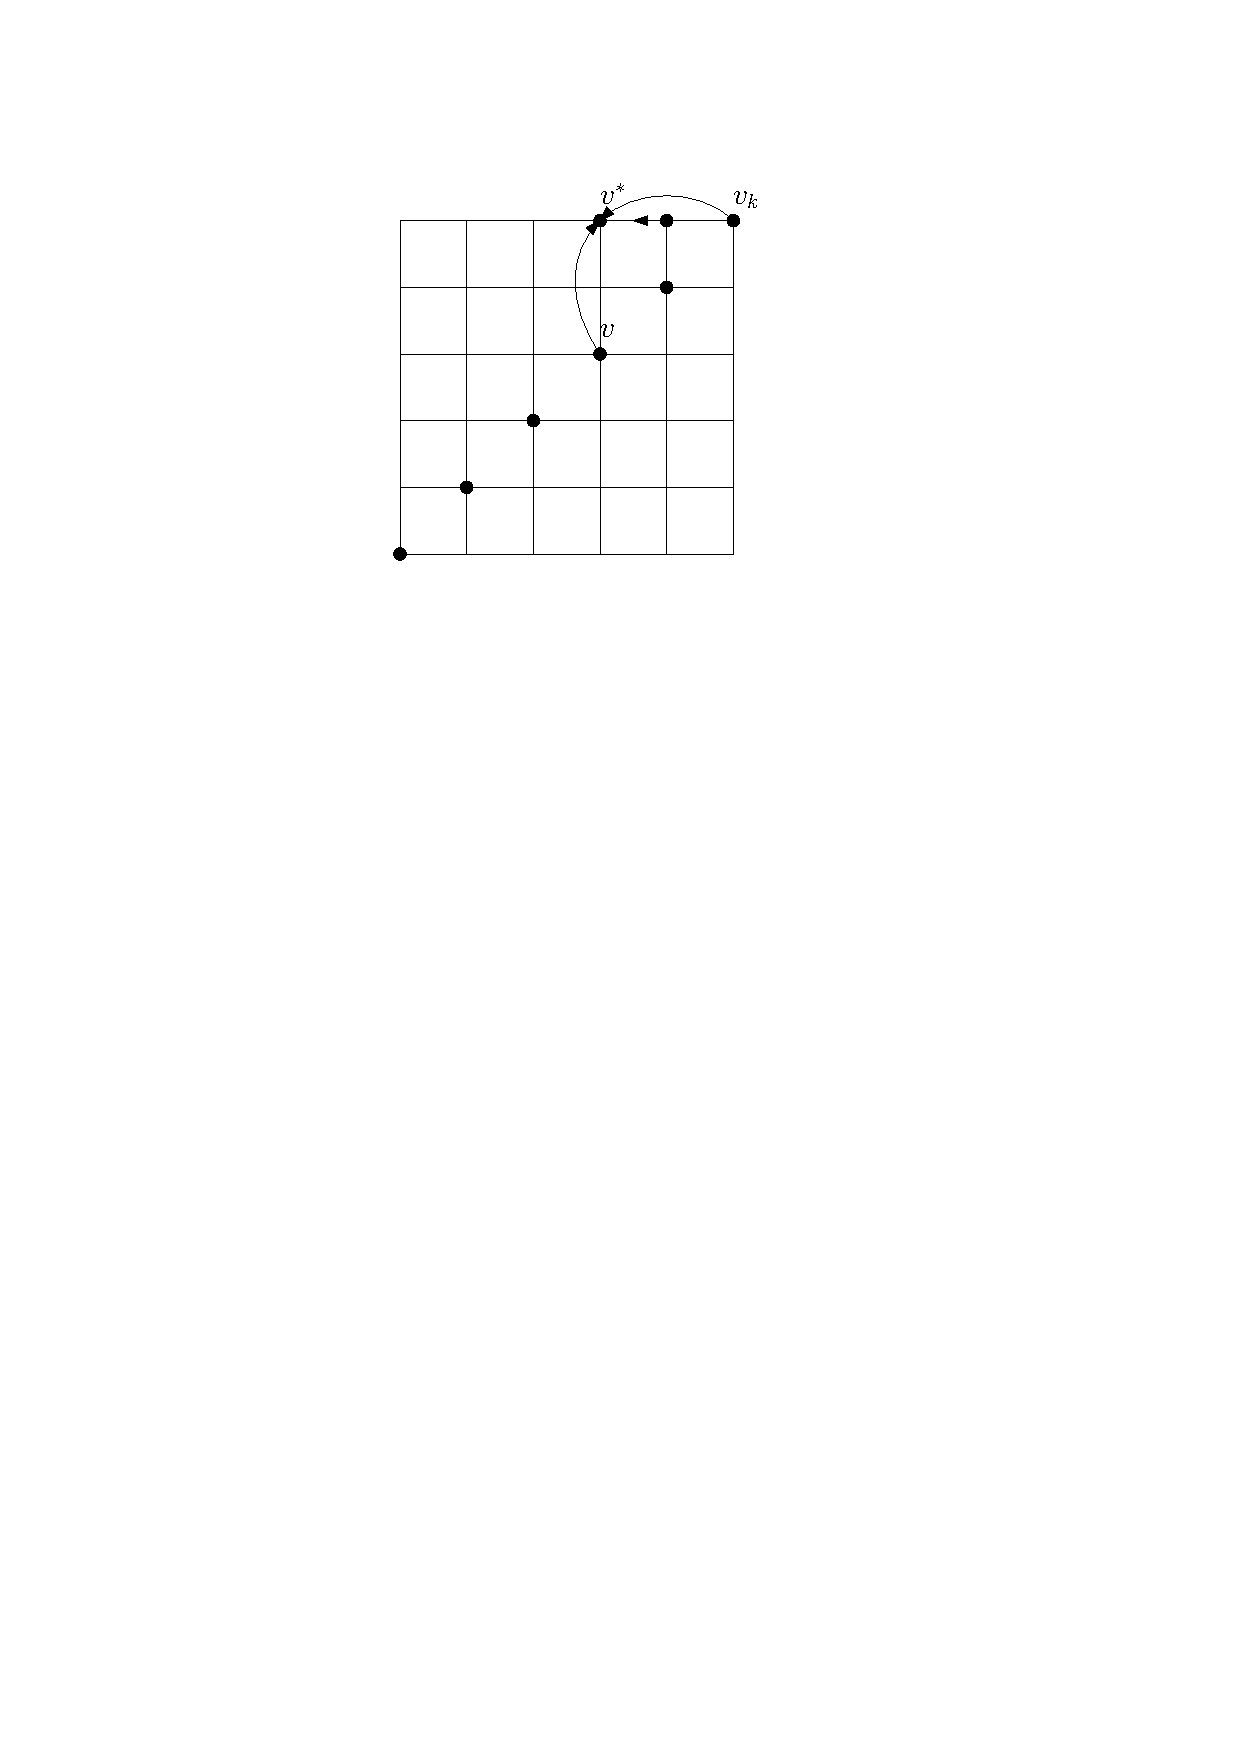
\includegraphics[scale=0.7]{seedlemma_fig1.pdf}
  %	\caption{In this figure only a subset of the edges of the grid appears. The vertices that are marked with discs are the ones evaluated.} 
  %	\label{fig:seedlem1}
  %\end{figure}
   %If we can show that there is an edge from $w$ to $v^*$, then by acyclicity $v^*$ has at least one more incoming vertical edge as compared to $w$, therefore establishing that $b \geq \frac{\lceil \frac{n}{2}\rceil-1}{2} + 1 \geq \frac{n}{4} \geq \frac{n}{4} - 1$ and showing that$v^*$ is an $(\frac{n}{4}, \frac{n}{4})$-vertex. 
   
   %Because $v$ is a minimal vertex in $V'$, either $w\succeq v$, or $v$ and $w$ are incomparable. 
   %To show that there is an edge from $w$ to $v^*$ we study these two cases: 
   %\MM{If I'm following this correctly, then the case distinction is
   %unnecessary. An edge $v^* \to w$ would immediately contradict $v
   %\not\succeq w$.}
   %If $w \succeq v$, then because $v \succeq v^*$ we have due to transitivity that $w \succeq v^*$. 
  %Otherwise, $w$ and $v$ are incomparable. In this case, since $v^*$ is smaller than $v$, we know %that the edge connecting $v$ and $v^*$ is  oriented towards $v^*$. 
  %Therefore, the only possibility for $v$ and $w$ to be incomparable is that there is an edge from $w$ to $v^*$. 
  %We give illustrations of the two cases in Figure~\ref{fig:seedlem2}. 
  %Thus regardless of the case, there is an edge from $w$ to $v^*$ which concludes the proof. \qed  
  % \begin{figure}[htbp] 
  %     \centering
  %     \begin{subfigure}[b]{0.4\textwidth}
  %         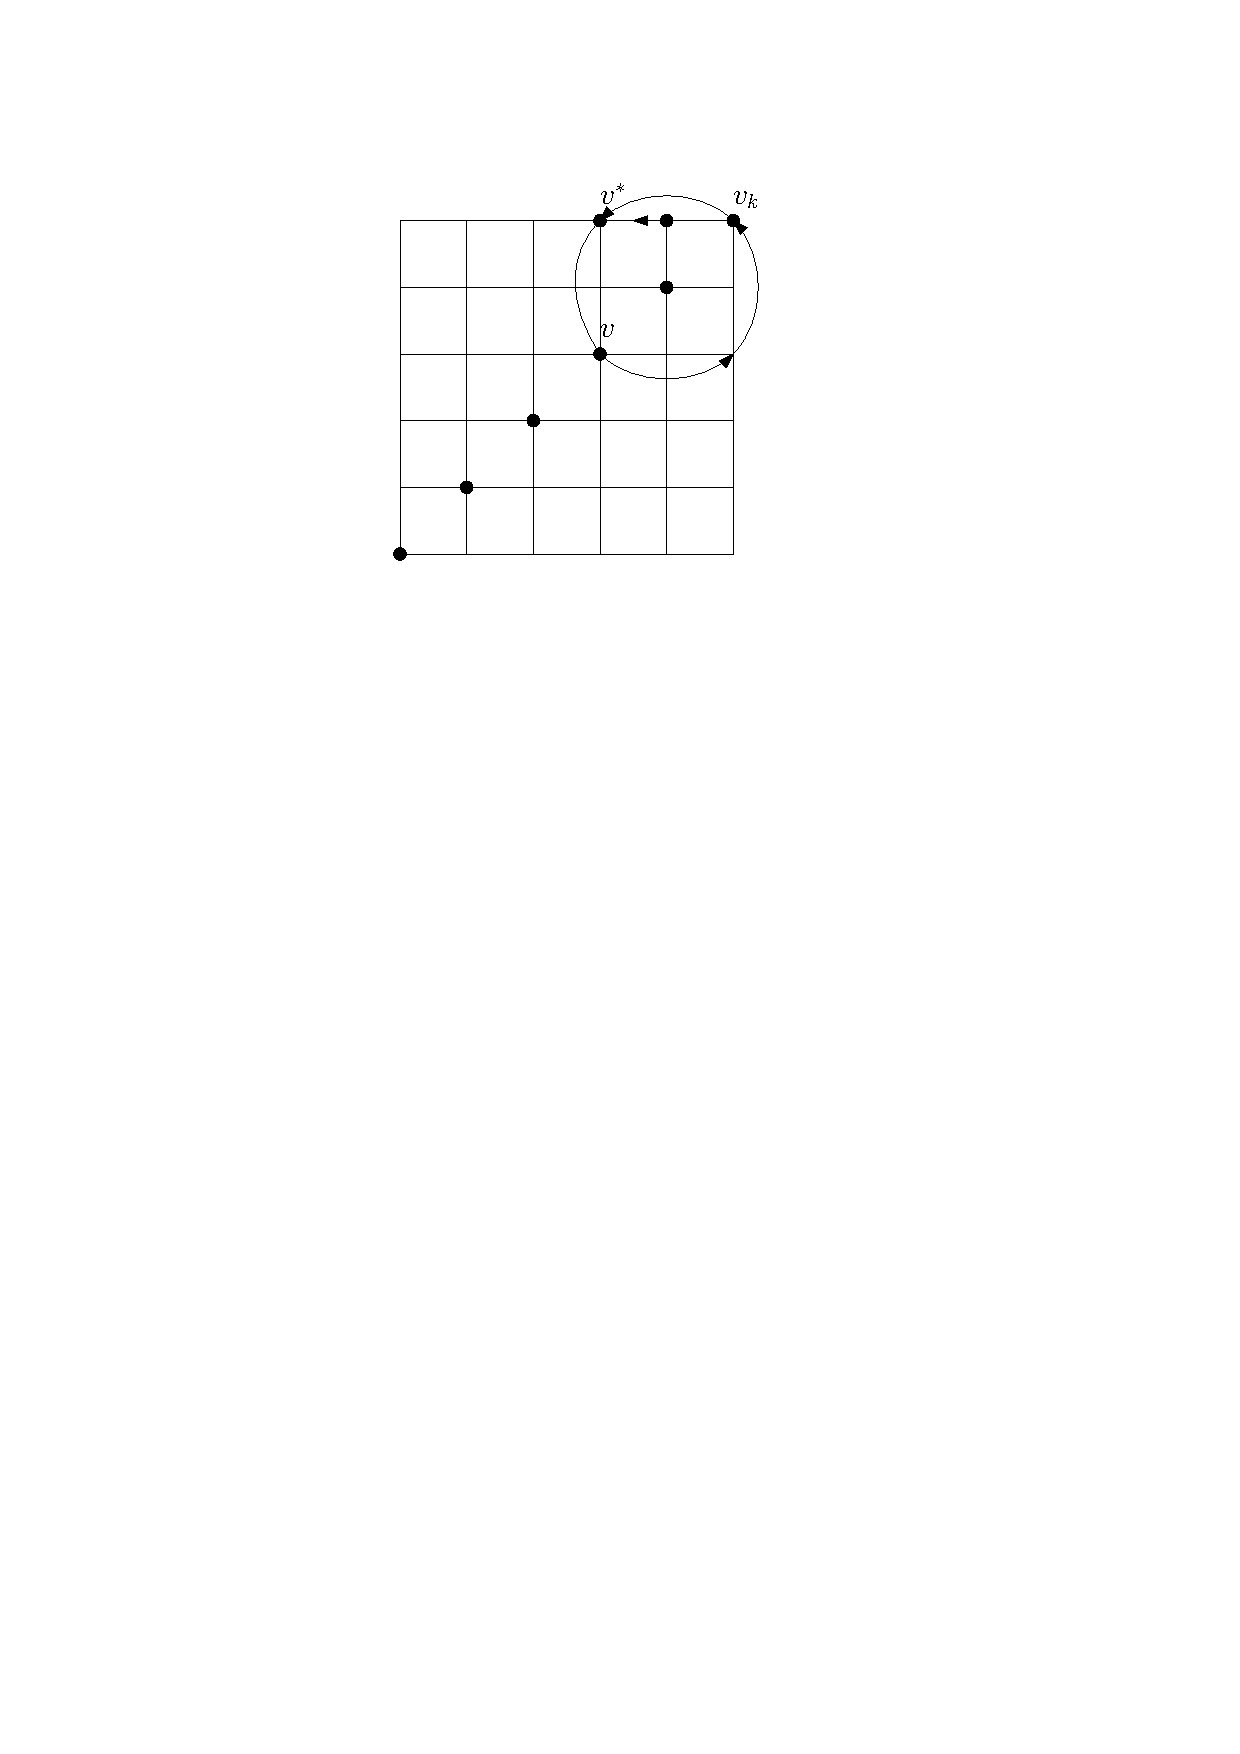
\includegraphics[scale = 0.7]{seedlemma_fig2_cas1.pdf}
  %         \caption{$w \succeq v$}
  %     \end{subfigure}
  %     \qquad \qquad
  %     \begin{subfigure}[b]{0.4\textwidth}
  %         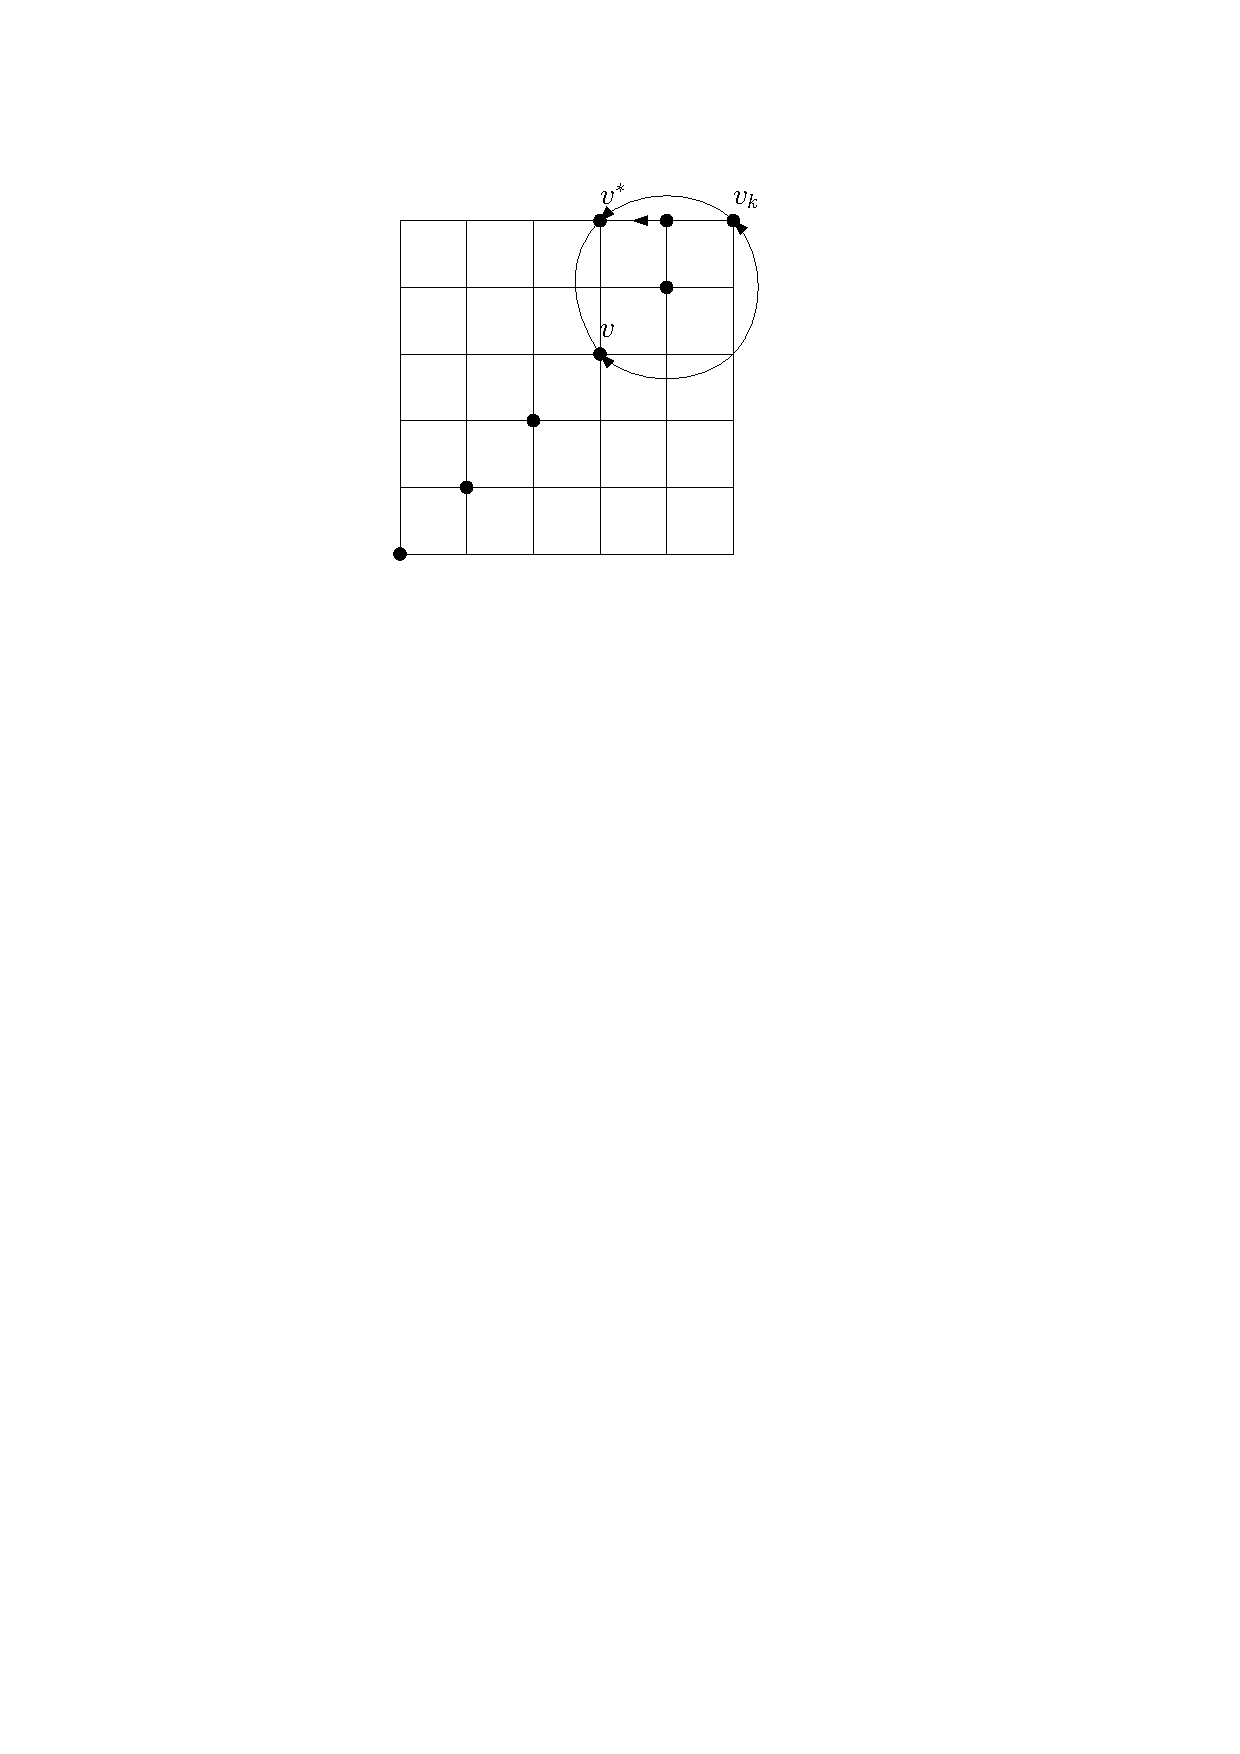
\includegraphics[scale = 0.7]{seedlemma_fig2_cas2.pdf}
  %         \caption{$v$ and $w$ are incomparable}
  %     \end{subfigure}
  %     \caption{Illustrations of the two cases. }
  %     \label{fig:seedlem2}
 %  \end{figure}
\end{proof}

The following corollary extends the previous lemma to non-square grids.

\begin{corollary}\label{corollary: n/4 indegree}
  Given an $[m]\times [n]$ grid USO $G$, we can find a vertex with \indegree $[a,b]$ with $a \geq \frac{m}{8} - 1$ and  $b \geq \frac{n}{8} - 1$ using $\mathcal{O}(M)$ vertex queries where $M = \max\{m,n\}$.
\end{corollary}

\begin{proof}
 Assume without loss of generality that $m \geq n$. 
 We will partition $[m]$ into $n$ blocks, then apply Lemma~\ref{lem:seed_lemma_for_square_matrices} on the induced orientation, and conclude using Theorem~\ref{thm:the_sink_of_the_sink_of_the_induced_orientation_is_the_global_sink} that this  gives us the desired result.
 
  Let $\A$ be a partition of $[m]$ into $n$ blocks, each of size either $\left\lfloor \frac{m}{n} \right\rfloor$ or $\left\lceil \frac{m}{n} \right\rceil$. Let $\B = [n]$ and 
consider the $\A$-$\B$-partition grid $H = K_\A\times K_\B$ and its induced orientation inherited from $G$. 
 Use Lemma~\ref{lem:seed_lemma_for_square_matrices} to find an $(\frac{n}{4}, \frac{n}{4})$-vertex $v$ in $H$. 
 Note that in each vertex query of $H$ we need to find the sink of a $(|A|,1)$-grid for some $A\in \A$. 
 The total number of vertex queries of $G$ used is therefore $\mathcal{O}(\frac{m}{n}\cdot n) = \mathcal{O}(m)$ as asserted. 
 Since $v$ has at least $\frac{n}{4} - 1$ horizontal incoming edges in $H$, each of which is a $(|A|,1)$-grid in $G$ for some $A\in \A$, 
 by Theorem~\ref{thm:the_sink_of_the_sink_of_the_induced_orientation_is_the_global_sink} $v$ has at least $$\left(\frac{n}{4} - 1\right)\cdot\left\lfloor \frac{m}{n} \right\rfloor + \left\lfloor \frac{m}{n} \right\rfloor - 1 \geq \frac{m}{8} - 1$$ incoming edges in $G$.
 Vertex $v$ also has at least $\frac{n}{4} - 1 \geq \frac{n}{8} - 1$ incoming vertical edges which concludes the proof. \qed
\end{proof}


%if every induced directed subgraph that is attained by fixing or limiting the range of some coordinates of the vertices has a unique sink. More specifically, we require this property to hold for subgraphs that are attained by taking $d$ nonempty index sets $\emptyset \not= J_i \subseteq \mathbb{Z}_n, i = 1,\ldots,d$ and considering the induced subgraph over the vertices $\{(a_1,\ldots, a_d) \in V \: : \:  a_i \in J_i \: \forall i = 1,\ldots, d \}$. If each $J_i$ is the whole of $\mathbb{Z}_n$ or a singleton, we call the resulting induced subgraph a \emph{face}. The dimension $d' \in \{0,1,\ldots, d\}$ of the face is the number of index sets that are the whole of $\mathbb{Z}_n$. Note that a face of $(K_n)^d$ of dimension $d'$ is isomorphic to $(K_n)^{d'}$. Any face can be compactly written as a vector $(v_1,\ldots,v_d) \in \left(\mathbb{Z}_{n} \cup \{*\}\right)^d$ where $v_i$ matches the only element of $J_i$ when $J_i$ is a singleton and $v_i$ is $*$ otherwise. Unless otherwise clear, one should also specify what $n$ is when talking of faces. This concept of a face is a natural generalization from the $d$-cube $(K_2)^d$ for which the faces we defined correspond to the faces of the $d$-cube in the geometric sense.

%Consider some USO of $(K_n)^d$. For this USO we define the \emph{in-map} $\phi : V \rightarrow \mathbb{Z}_n^d$ for each vertex $v = (v_1,\dots, v_d) \in V$ so that $\phi(v)_i$ is the number of edges that are incoming for $v$ from its neighbors $w \in V$ that differ from $v$ on coordinate $i$. It was shown by \citet[Theorem 2]{gartner2008unique} that for a USO this mapping is infact a bijection. The \emph{product construction} for grids (\citet{gartner2008unique}, \citet{szabo2001unique}) states that we can contract dimensions and maintain the USO structure. More specifically, for any $I \subseteq \mathbb{Z}_n$ consider the set of faces 
% \begin{align*}
%  G = \{(a_1,\ldots,a_n) : a_i = * \textnormal{ if } i \in I \textnormal{ and } a_i \in \mathbb{Z}_n \textnormal{ otherwise}\}.
% \end{align*}
% Note that $|G| = n^{d-|I|}$ and there is a natrual way to consider a USO over a graph whose vertices are the faces in $G$: for any $f \in G$ its neighbors are those faces that differ from it in the fixed coordinates and the orientation of the edges is determined by the orientation of the corresponding edges in the sink of $f$. This definition turns out to be well defined and the arising structure forms a USO that is over a graph isomorphic to $(K_n)^{d-|I|}$. 
% 
% 
% The problem we are looking at is that of finding the global sink of a USO over $(K_n)^d$. The USO is given by an oracle that for any given vertex reveals the orientations of the edges adjacent to the vertex. The question is, what is the least number of these vertex queries needed to find the unique global sink? Just knowing its location is not sufficient, but we also require that the sink is evaluated. This requirement will prove useful when developing an algorithm.

\subsubsection{Finding an $(\frac{n}{2}, \frac{n}{2})$-vertex}

Given an $(a, b)$-vertex $v = (x_v, y_v)$ in an $[m]\times [n]$-grid USO, let $I_v\subseteq [m]$ be the set of indices such that  $I_v \times \{y_v\}$ is the set of all vertices with an outgoing horizontal edge to $v$ with $v$ included in this set. Analogously, $J_v\subseteq [n]$ is the set of indices such that $\{x_v\}\times J_v$ is the set of all vertices with an outgoing vertical edge to~$v$ (including $v$). Notice that $|I_v| = a$ while $|J_v| = b$.

\begin{observation}\label{Obs:Sink of dominated grid}
Given a vertex  $v = (x_v, y_v)$ in a grid USO, $v$ is the sink of the $I_v\times J_v$-grid.
\end{observation}
\begin{proof}
Vertex $v$ has only incoming edges in the $I_v\times J_v$-grid and is therefore the unique sink of this subgrid. \qed
\end{proof}

An \emph{$(\alpha, \beta)$-oracle} is an algorithm that, given an $(m, n)$-grid USO as input, can find an $(\alpha m, \beta n)$-vertex $v$ using $O(n + m)$ queries.

\begin{lemma}\label{lemma:Climbing lemma}
Let $G$ be an $[m]\times [n]$-grid USO.
Given an $(\alpha, \beta)$-oracle such that $0 < \alpha, \beta  < 1$, we can find both an $(\frac{m}{2}, \beta n)$-vertex and an $(\alpha m, \frac{n}{2})$-vertex in $G$ using $O(1)$ oracle calls and $O(n+m)$ additional vertex queries.
\end{lemma}
\begin{proof}
We show how to find an $(\alpha m,  \frac{n}{2})$-vertex. The procedure to find an $( \frac{m}{2}, \beta n)$-vertex is analogous.
Let $B_0 = [n]$ and let $G_0$ be the $[m]\times B_0$-grid, i.e., $G = G_0$.
Using an oracle call in $G_i$ (initially $i = 0$), find an $(\alpha n, \beta n)$-vertex $v_i$ in $G_i$. 
Recall that $v_i$ is the sink of the $I_{v_i}\times J_{v_i}$-grid by Observation~\ref{Obs:Sink of dominated grid}.
Notice that $|I_{v_i}| \geq \alpha m$ while $|J_{v_i}| \geq \beta |B_i|$.
Let $B_{i+1} = B_i\setminus J_{v_i}$ and let $G_{i+1}$ be the $[m]\times B_{i+1}$-grid. 
Repeat this procedure with $G_{i+1}$ as long as $|B_i| \geq  \frac{n}{2}$; see Figure~\ref{fig:Climbing Lemma}.

\begin{figure}[h]
\centering
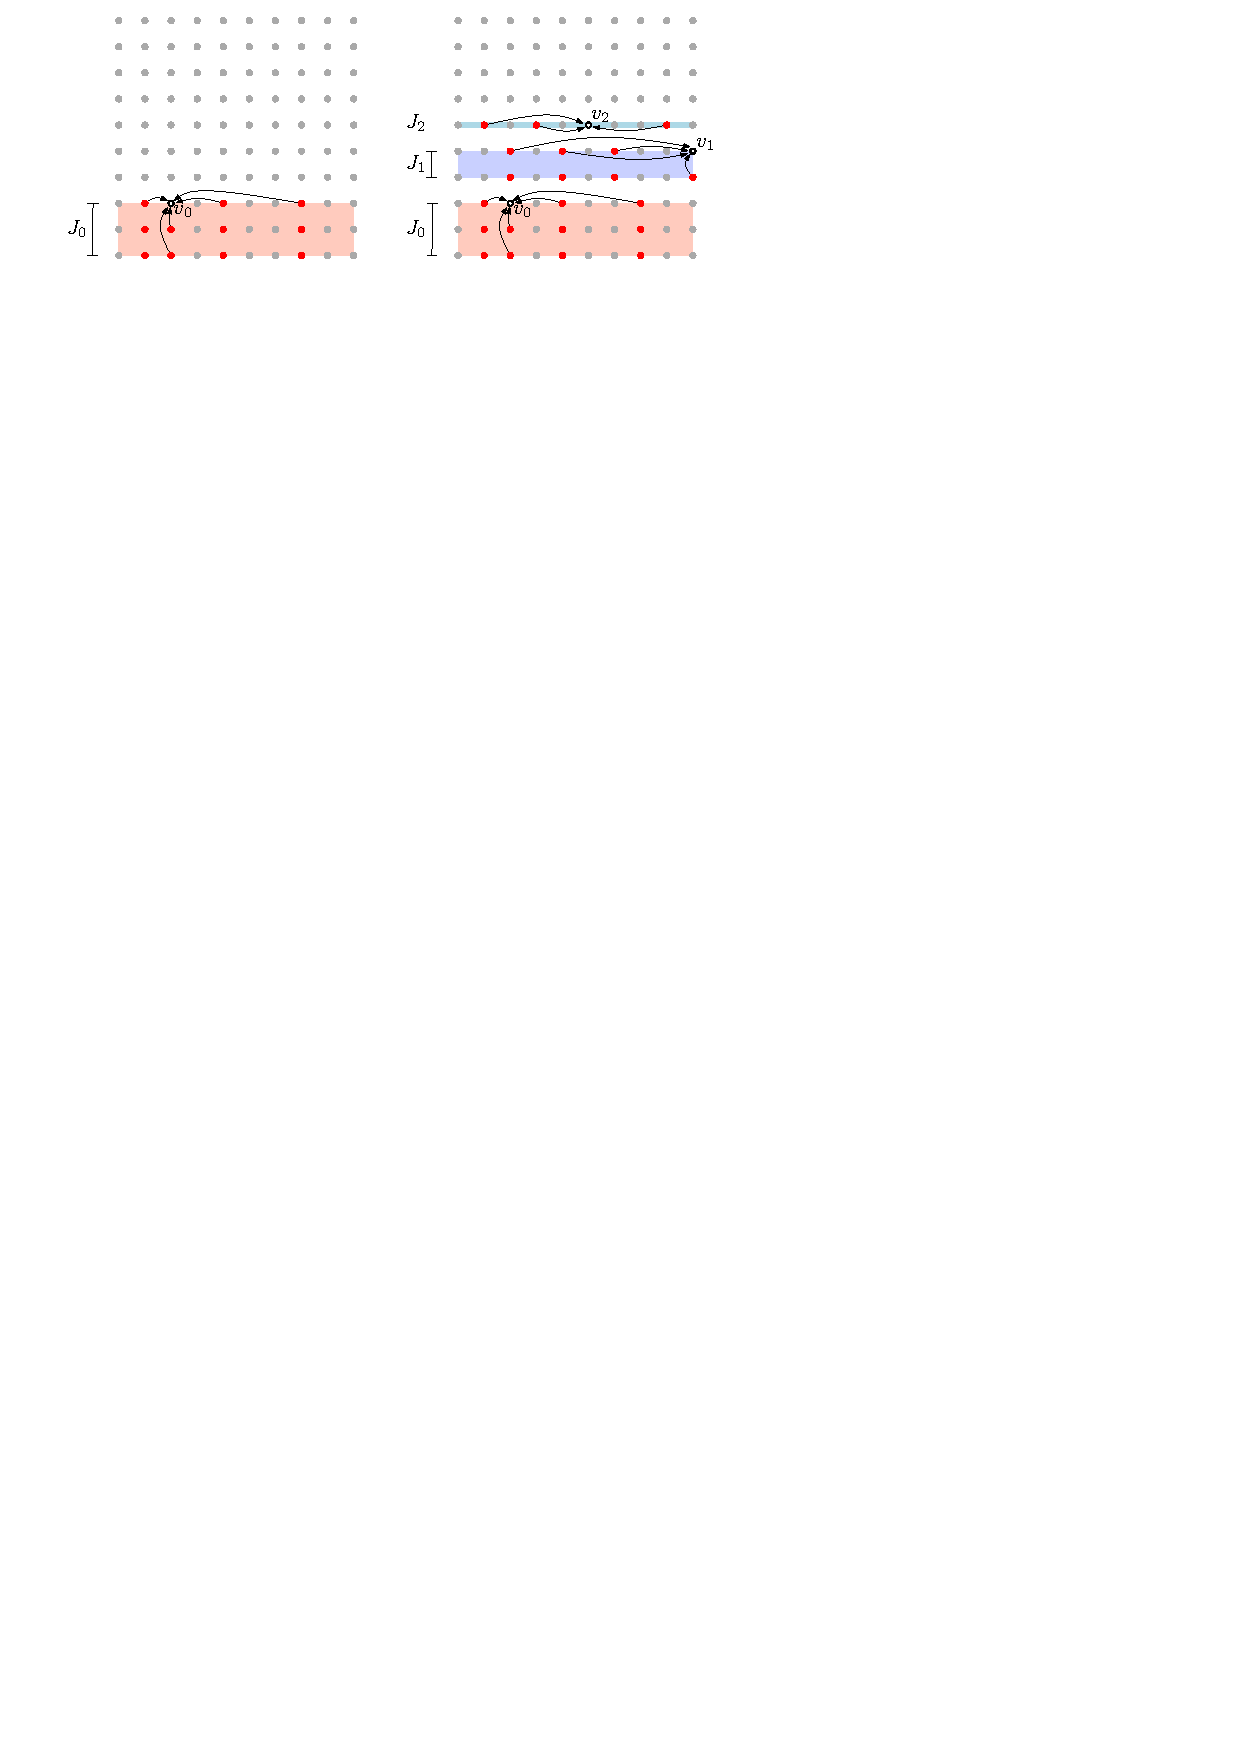
\includegraphics[width=1\textwidth]{ClimbingLemma.pdf}
\caption{\small }
\label{fig:Climbing Lemma}
\end{figure}

Since $0 < \beta < 1$, after $k = O(1)$ iterations, the above procedure stops. 
Because the process stopped, we know that $|B_{k+1}| = |B_k \setminus J_{v_k}| <  \frac{n}{2}$.
Since $B_{k+1} = B_0\setminus \cup_{i=0}^k J_{v_i}$, we know that $|\cup_{i=0}^k J_{v_i}| >  \frac{n}{2}$.

Let $H$ be the smallest subgrid that contains the vertices $v_0, \ldots, v_k$. Since $k = O(1)$, $H$ consists of a constant number of vertices. Therefore, we can find its sink $s$ using $O(1)$ operations. 
Assume that $s = (x_s, y_s)$ and let $s'$ be the sink of the $\{x_s\}\times \cup_{i=0}^k J_{v_i}$-subgrid. 
Let $h$ be such that $s'$ belongs to the $[m]\times J_{v_h}$-subgrid; see Figure~\ref{fig:Climbing Lemma-2}.

\begin{figure}[h]
\centering
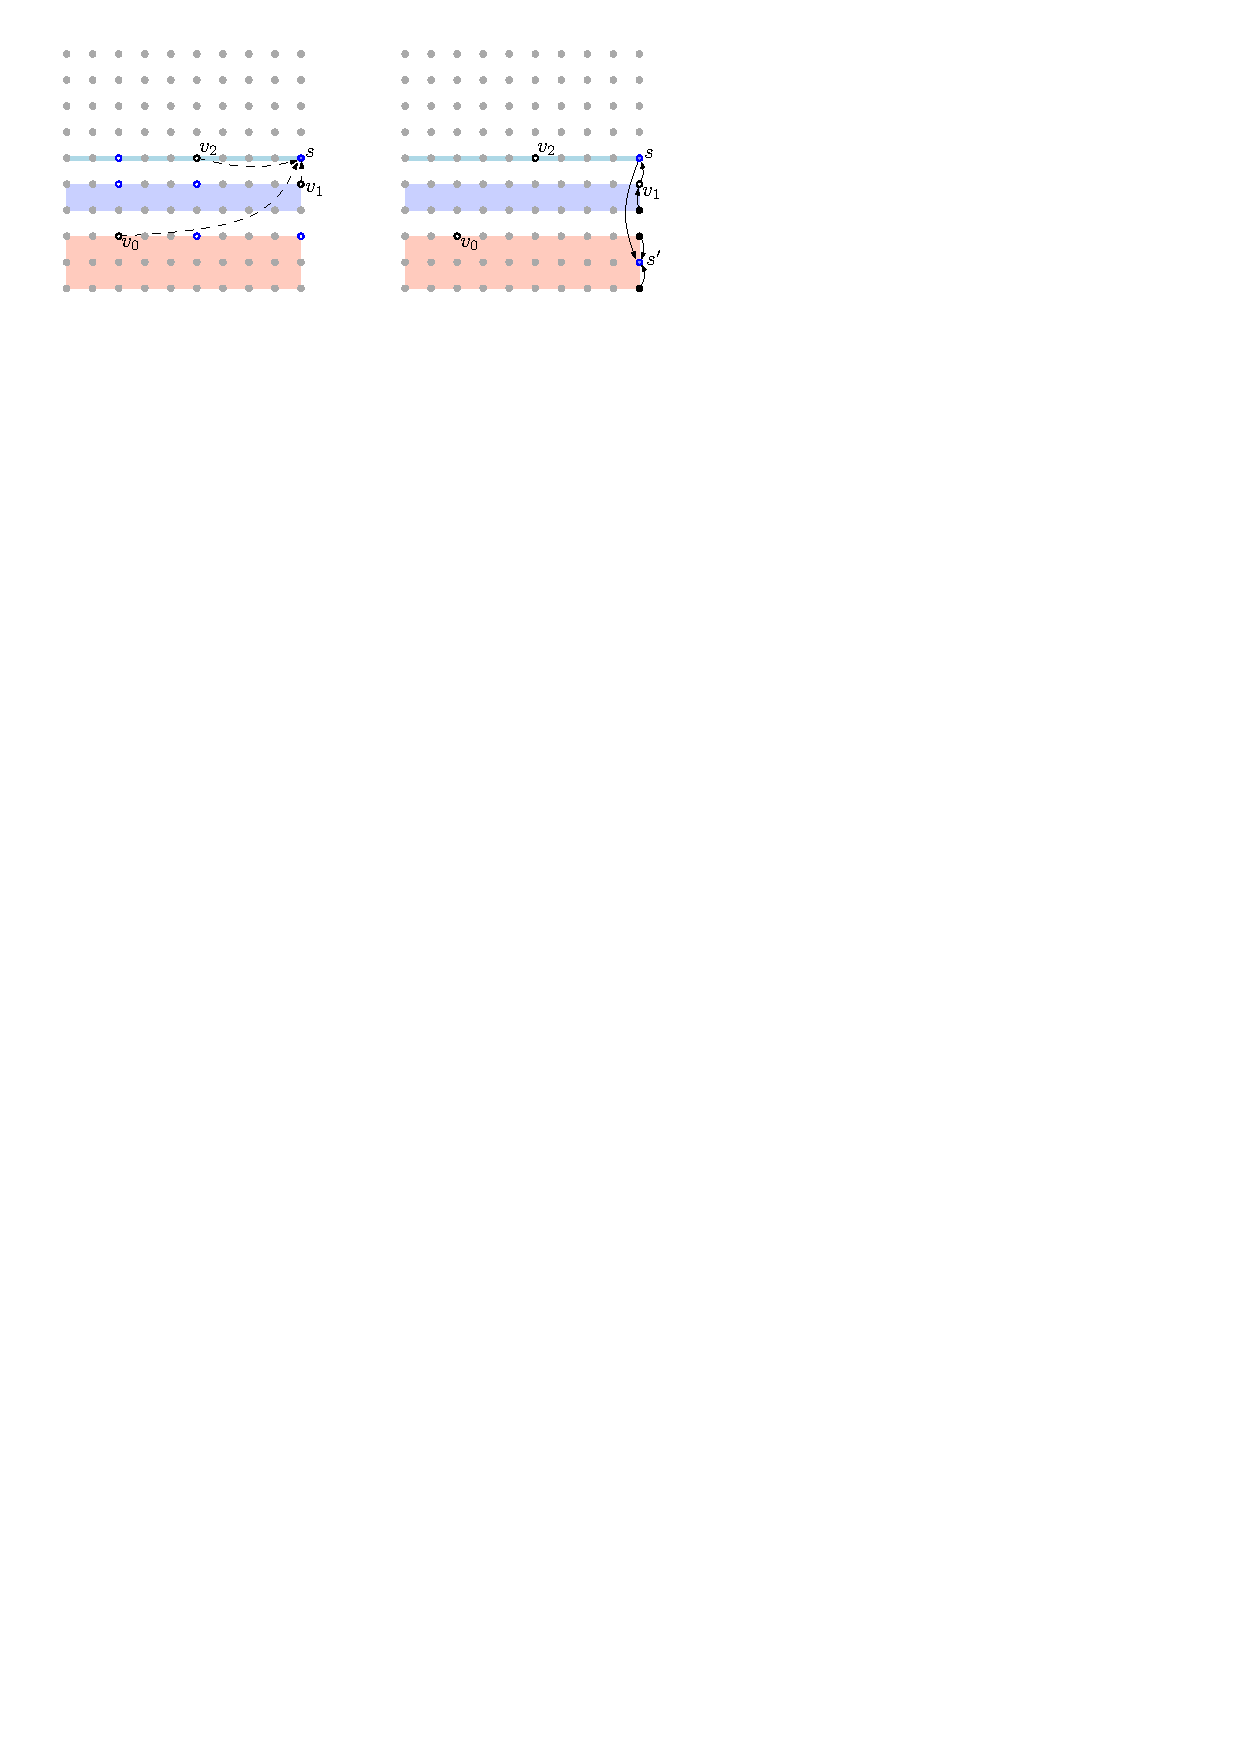
\includegraphics[width=1\textwidth]{ClimbingLemma-2.pdf}
\caption{\small }
\label{fig:Climbing Lemma-2}
\end{figure}

Let $[a,b]$ be the \indegree of $s'$.
Recall that $s$ is smaller than $v_h$, hence $s'$ is also smaller than $v_h$.
Because $v_h$ is the sink of the $I_{v_h}\times J_{v_h}$-grid, $s'$ is smaller than each vertex in the $I_{v_h}\times J_{v_h}$-grid.
Therefore, at least $|I_{v_h}|$ vertices have outgoing edges to $s'$ in the row containing $s'$, i.e., $a\geq |I_{v_h}| \geq \alpha m$.
Moreover, since $s'$ is the sink of the $\{x_s\}\times \cup_{i=0}^k J_{v_i}$-subgrid, $b \geq |\cup_{i=0}^k J_{v_i}|  >  \frac{n}{2}$.
Consequently, $s'$ is an $(\alpha m,  \frac{n}{2})$-vertex. \qed
\end{proof}

\begin{corollary}\label{corollary: (m/2,n/2) indegree}
Let $G$ be an $[m]\times [n]$-grid USO. 
We can compute an $( \frac{m}{2}, \frac{n}{2})$-vertex using $O(n + m)$ vertex queries.
\end{corollary}
\begin{proof}
Notice that Corollary~\ref{corollary: n/4 indegree} proves the existence of an $( \frac{1}{8}, \frac{1}{8})$-oracle.
We use Lemma~\ref{lemma:Climbing lemma} with the $(\frac{1}{8}, \frac{1}{8})$-oracle as input, to find an $(\frac{m}{8}, \frac{n}{2})$-vertex using only $O(1)$ calls to this $(\frac{1}{8}, \frac{1}{8})$-oracle and $O(n+m)$ additional vertex queries. Since each call to the  $(\frac{1}{8}, \frac{1}{8})$-oracle can be implemented with $O(n+m)$ vertex queries by Corollary~\ref{corollary: n/4 indegree}, the algorithm to find the $(\frac{m}{8}, \frac{n}{2})$-vertex is a $(\frac{1}{8}, \frac{1}{2})$-oracle. 
Therefore, using again Lemma~\ref{lemma:Climbing lemma} with this $(\frac{1}{8}, \frac{1}{2})$-oracle as input, we can find an $(\frac{m}{2}, \frac{n}{2})$-vertex using $O(1)$ calls to the $(\frac{1}{8}, \frac{1}{2})$-oracle. That is, in total $O(n + m)$ queries suffice to find an $(\frac{m}{2}, \frac{n}{2})$-vertex. \qed
\end{proof}


We are ready to state our main result. 
\begin{theorem}\label{theorem:Sink algorithm}
 Let $M = \max\{m,n\}$. The sink of an $[m]\times[n]$-grid USO can be found after $\mathcal{O}(M(\log M))$ vertex queries.
\end{theorem}
\begin{proof}
Use Corollary~\ref{corollary: (m/2,n/2) indegree} to find an $(\frac{m}{2}, \frac{n}{2})$-vertex $v$. 
Recall that $v$ is the sink of the $I_v\times J_v$-grid by Observation~\ref{Obs:Sink of dominated grid}, where $|I_v| \geq \frac{m}{2}$ and $|J_v|\geq \frac{n}{2}$. Let $A_1\subset I_v$ and $B_1\subset J_v$ be subsets of indices such that $|A_1| = \frac{m}{2}, |B_1| = \frac{n}{2}$ and $v\in A_1\times B_1$-subgrid.
Let $A_2= [m]\setminus A_1$ and $B_2 = [n]\setminus B_1$.
Let $\A = \{A_1, A_2\}$ and $\B = \{B_1, B_2\}$ be partitions of $[m]$ and $[n]$, respectively.

Let $T(m, n)$ be the number of queries needed to find the sink of an $[m]\times[n]$-grid USO.
We can find recursively the sink $s$ of the $A_2\times B_2$-subgrid using $T(\frac{m}{2}, \frac{n}{2})$ vertex queries. 
If neither $v$ nor $s$ is the sink of $G$ we proceed as follows.
Since the orientation of the $\A$-$\B$-partition grid $H = K_\A \times K_\B$ induced by $G$ is a unique sink orientation by Lemma~\ref{lemma:USO-Lemma}, we can decide whether the sink of $G$ lies in the $A_1\times B_2$-grid or in the $A_2\times B_1$-grid after querying $v$ and $s$. Assume without loss of generality that it lies in the $A_1\times B_2$-grid.
By finding recursively the sink of the $A_1\times B_2$-grid, we find the sink of $G$ by Theorem~\ref{thm:the_sink_of_the_sink_of_the_induced_orientation_is_the_global_sink}. In summary, the total number of queries requried to find the sink of $G$ is given by the recurrence
$$T(m, n) = 2\cdot T\left(\frac{m}{2}, \frac{n}{2}\right) + O(n+m),$$
which solves to $T(m, n) = O((n+m) \log (n+m))$ yielding our result. \qed
\end{proof}
 
\subsection{A Deterministic Lower Bound}
\label{section:a_deterministic_lower_bound}

We give a linear lower bound on the number of vertex queries required to find
the sink of an $(m,n)$-grid USO.
More precisely, we will see that
\[
    \timeVertex(N) \ge N-1
\]
where, as before, $N = m+n$.

We begin with the case $n=1$, where the grid consists of a single row:

\begin{lemma}\label{lem:kx1}
Every deterministic algorithm needs $m$ queries to find the sink of an $(m,1)$-grid USO.
\end{lemma}
\begin{proof}
    The proof proceeds by an adversary argument.
    We thus consider a game played between the algorithm (which successively
    queries vertices) and the adversary (who answers the queries),
    and we claim that the adversary has a strategy which allows him to enforce
    that the algorithm does not query the sink before the $m$th query.

Let $v_i$ denote the vertex evaluated at the $i$-th query, for $i=1,\ldots, m$. At evaluation of $v_1$ we answer with the global source. Then, at every vertex
we answer with all edges that are not yet defined to be outgoing. Then, $v_i$ has $i-1$ incoming edges, already evaluated from the previous evaluations. 
Therefore, $v_i$ has $m-i$ outgoing edges. At the $(m-1)$-th iteration the vertex $v_{m-1}$ will have one outgoing edge which will point to $v_m$.
The algorithm then needs to also evaluate $v_m$ (which will be the sink) for a total of $m$ queries. \qed 
\end{proof}

\begin{theorem} \label{thm:lowerbound}
Every deterministic algorithm needs at least $m+n-1$ queries to find the sink of a $(m,n)$-grid USO. 
\end{theorem}
\begin{proof}
    This proof again proceeds by an adversary argument.

Let $A$ be a sink-finding algorithm. We say that $A$ \emph{explores} a row of $G$ whenever it queries a vertex in this row for the first time.
Each time $A$ explores an unexplored row, we label this row with the smallest unused label from the set $\{1, \ldots, n\}$. Moreover, we assign an arbitrary order to the vertices in this row and reveal any queried horizontal edge in this row according to this order. For the vertical edges between explored rows, we simply follow the rule that a vertex in the row labeled $i$ is always smaller than any vertex in the row labeled $j$, for any $i > j$. Additionally, a vertex in a labeled row is always larger than any vertex in an unexplored row. In other words, we determine a lexicographical total order on the vertices of the gird. One can think of each vertex in an explored row as having two coordinates: the first being the label of its row, and the second the rank of this vertex in its row.
It is easy to check that the answers are consistent with a unique sink orientation.

Because vertices in unexplored rows are always smaller, the sink of $G$ lies always in an unexplored row throughout the execution of $A$. Therefore, $A$ requires at least $n$ vertex queries before querying the first vertex in the row $r$ containing the sink. Once $A$ has queried the first vertex in $r$, it has still to find the maximum among its $m$ vertices. 
By Lemma~\ref{lem:kx1} this requires at least $m$ vertex queries of which the algorithm has performed exactly one. Thus, $m-1$ additional vertex queries are needed to find the sink. That is, $A$ requires at least $n+m-1$ vertex queries to find the sink of $G$. \qed
\end{proof}

A unique sink orientation is called \emph{combed} in rows (columns) if the orientation of all the edges between the vertices of any two rows (columns) are the same. 
A combed USO is combed either in the rows or in the columns. The unique sink orientation arising in the proof of Theorem~\ref{thm:lowerbound} is an example of a USO that is combed in the rows.
The next theorem shows that if one wants to improve the lower bound of Theorem~\ref{thm:lowerbound}, it is not sufficient to consider only combed USOs.

\begin{theorem}
 The sink of a combed $(m,n)$-grid USO can be found by using $n+m-1$ vertex queries.
\end{theorem}

\begin{proof}
 If we know that the grid is combed in rows or columns, then the same approach used by the adversary player in the proof of Theorem~\ref{thm:lowerbound} will work.
 If we don't know the direction of the combing, there is a strategy that will find the sink within the required number of steps: after querying a vertex, the next vertex to be checked is the one that is the furthest away from the current vertex within the subgrid that is spanned by the edges leaving the curent vertex. 
 
 This strategy works because no matter in which direction the USO is combed, at every step we discard  one or more of the irrelevant rows or columns. For example, if the USO is combed in rows, then in at most $n$ queries we will be at a vertex that has only horiontal outgoing edges. That is, we have found the row where the sink is in. In the next $m-1$ all queries will be in that row so that in the required number of queries we have found the sink. \qed
\end{proof}


\subsection{Optimality of the Lower Bound for Small Grids}

We now write $\timeVertex(m,n)$ for the minimum number of queries that a
deterministic algorithm must ask in the worst case to find and query the sink
in a grid $G = K_m \times K_n$.
Here we analyze some small cases:
\begin{theorem}
    \label{thm:smallGrids}
    Let $n \le 4$. Then $\timeVertex(n,n) = 2n-1$.
\end{theorem}
Thus we will find that for the cases covered by the theorem, the lower bound
in Theorem~\ref{thm:lowerbound} is tight.

We omit the proofs for the cases $n = 1,2,3$. Namely,
\begin{itemize}
    \item
        if $n \le 2$ then the graph $G = K_n \times K_n$ coincides with the
        ``$n$-cube'', already discussed to large extents in the USO
        literature;
    \item
        and if $n = 3$ then the proof is similar to the case $n=4$, but much
        simpler.
\end{itemize}
The rest of this subsection will thus be concerned with the following
proposition, whose proof will settle Theorem~\ref{thm:smallGrids}.

\begin{proposition}
    \label{prop:4:7}
    There is a deterministic algorithm which queries the sink in a
    $(4,4)$-grid USO and which uses at most 7 vertex queries.
\end{proposition}

For the description of the algorithm we introduce some terminology:
An edge of the grid has been \emph{discovered} if an incident vertex has been
queried.
At any step of the algorithm, a vertex of the grid can be either \emph{alive}
or \emph{dead}.
These adjectives obey the following rules:
\begin{itemize}
    \item
        In the very beginning, every vertex is alive; and in the very end, the
        sink is the only vertex that is still alive.

    \item
        A vertex changes its state at most once.
        In other words, a vertex can die, but it cannot come to life again.
\end{itemize}
We begin by stipulating two obvious conditions under which we let a vertex die:
\begin{enumerate}
    \item
        An edge $u \to v$ is discovered. At this moment the vertex $u$ dies.

    \item
        The sink is queried. If at this moment there are still any other
        vertices alive, they die instantly.
\end{enumerate}

\begin{lemma}
    Let $(i,j)$ and $(k,l)$ be vertices of the grid that have already been
    queried, $i \neq k$, $j \neq l$.
    Then among the two vertices $(i,l)$ and $(k,j)$, at least one is dead.

    \label{lem:rectangle}
\end{lemma}

\begin{proof}
    The four vertices $(i,j)$, $(k,j)$, $(k,l)$, $(i,l)$ form a subgrid, a
    rectangle.
    The four edges of this rectangle have been discovered, and the rectangle
    contains a unique sink: hence, according to condition 1, at least three
    corners of the rectangle have died. \qed
\end{proof}

\begin{lemma}
    \label{lem:kill}
    Let $i \neq k$, $j \neq l$.
    Assume that
    \begin{itemize}
        \item the vertex $(i,j)$ has been queried,
        \item the vertex $(k,l)$ has died \emph{from condition 1}.
    \end{itemize}
    Then for one of the two vertices $(i,l)$ and $(k,j)$ it is already known
    that it cannot be the sink: and thus our algorithm is allowed to ``kill''
    this vertex, unless it has already died before.
\end{lemma}

\begin{proof}
    By lemma \ref{lem:rectangle} we can assume that $(k,l)$ has not been
    queried.
    Now assume furthermore that neither $(i,l)$ nor $(k,j)$ is dead.

    Then we have already discovered the edges $(i,j) \to (i,l)$ and $(i,j) \to
    (k,j)$.
    Since $(k,l)$ has died from condition 1, there must be a discovered edge
    $(k,l) \to u$ for some incident vertex $u$.
    We will assume without loss of generality that $u$ lies in the same row as
    $(k,l)$, and also that $u \neq (k,j)$:
    \begin{align*}
        \xymatrix{
            (i,j) \ar[d] \ar[r] & (i,l)
            \\
            (k,j) & (k,l) \ar[r] & u
        }
    \end{align*}
    We have assumed that $(k,l)$ has not been queried; then $u$ must have been
    queried so as to discover the edge $(k,l) \to u$.
    Hence, $u \to (k,j)$, for otherwise $(k,j)$ would already have died.
    This implies $(k,l) \to (k,j)$ due to acyclicity (cf.~lemma
    \ref{lemma:acyclicity_lemma}).
    But then $(k,j)$ is the unique sink of the subgrid
    $\{i,k\} \times \{j,l\}$,
    and thus $(i,l)$ cannot be a sink. \qed
\end{proof}

As a consequence of lemma \ref{lem:rectangle} we can observe that,
if the four vertices on the diagonal of the $(4,4)$-grid have already
been queried, then at least 10 vertices have died.
Motivated by this observation, our algorithm will start out by querying
the four vertices on the diagonal.
Having done this, let us characterize the resulting situation by putting some
labels on the vertices of the grid:
\begin{itemize}
    \item
        The four vertices of the diagonal we label by ``$0$'', so that we
        remember that we have already queried them.
    \item
        The 6 vertices that died according to lemma \ref{lem:rectangle} we label
        ``$+$''.
    \item
        If we put a ``$+$'' on vertex $(i,j)$, then we put a ``$-$'' on vertex
        $(j,i)$, be it dead or alive.
\end{itemize}
A grid thus labelled can e.\,g.~look like so:
\begin{align*}
    \begin{pmatrix}
        0 & - & - & +
        \\
        + & 0 & - & -
        \\
        + & + & 0 & -
        \\
        - & + & + & 0
    \end{pmatrix}
\end{align*}
Every such labelling is nothing but an antisymmetric $4 \times 4$-matrix with
entries in $\{0,+,-\}$, and with no zero entries except on the diagonal.
Let $X$ be the set of such matrices: we have $|X| = 2^6$.
Since we are not very keen on discussing each of these cases individually, we
will use the symmetry of the situation:

Let $G$ be the group $\Sym_2 \times \Sym_4$ and denote the generator of
$\Sym_2$ by $\tau$.
Let $G$ act on $X$ by
\begin{align*}
    (\tau,M) ~&\mapsto~ M^\Tr   && (M \in X),
    \\
    (\sigma,M) ~&\mapsto~ P_\sigma \, M \, P_\sigma^\Tr
            && (\sigma \in \Sym_4,~ M \in X).
\end{align*}
Here $P_\sigma$ denotes, for a permutation $\sigma \in \Sym_4$, the
permutation matrix determined by $P_\sigma e_i = e_{\sigma(i)}$, $i \in
\{1,2,3,4\}$.
Whenever two matrices are in the same orbit, they describe analogous cases for
our proof.
A quick computer search reveals that a system of representatives for our group
action is given by
\begin{align*}
    A =
        \begin{pmatrix}
            0 & - & - & -
            \\
            + & 0 & - & -
            \\
            + & + & 0 & -
            \\
            + & + & + & 0
        \end{pmatrix},
    \qquad
    B =
        \begin{pmatrix}
            0 & - & - & +
            \\
            + & 0 & - & -
            \\
            + & + & 0 & -
            \\
            - & + & + & 0
        \end{pmatrix},
    \qquad
    C =
        \begin{pmatrix}
            0 & - & - & -
            \\
            + & 0 & - & +
            \\
            + & + & 0 & -
            \\
            + & - & + & 0
        \end{pmatrix}.
\end{align*}

The theorem now follows from the
\begin{lemma}
    In each of the cases $A$, $B$, $C$ listed above, we can query the sink
    using at most another three vertex queries.
\end{lemma}

\begin{proof}[Proof of case $A$]
    The next (fifth) vertex that we query is the one in the upper right
    corner, $(1,4)$.
    By lemma \ref{lem:kill} we can now ``kill'' at least one vertex from
    the set $\{ (1,2), (3,4) \}$.
    Furthermore, by lemma \ref{lem:rectangle}, at least one vertex each from
    the following sets is dead: $\{ (1,2), (2,4) \}$
    and $\{ (1,3), (3,4) \}$.
    This leaves us with one of the following situations, where the ``$=$''
    marks the vertices that we have just recognized to be dead:
    \begin{align*}
        \begin{pmatrix}
            0 & = & = & 0
            \\
            + & 0 & - & -
            \\
            + & + & 0 & -
            \\
            + & + & + & 0
        \end{pmatrix},
        \quad
        \begin{pmatrix}
            0 & = & - & 0
            \\
            + & 0 & - & -
            \\
            + & + & 0 & =
            \\
            + & + & + & 0
        \end{pmatrix},
        \quad
        \begin{pmatrix}
            0 & - & - & 0
            \\
            + & 0 & - & =
            \\
            + & + & 0 & =
            \\
            + & + & + & 0
        \end{pmatrix}.
    \end{align*}
    In every case the vertices which are still alive (which we know to be a
    subset of the vertices marked ``--'') are contained in a
    square, one corner of which has already been queried.
    By lemma \ref{lem:rectangle} the sink of the square can be queried using
    at most two further queries, for a total of seven vertex queries.
    ---
    We omit the proof for case $B$ and case $C$; in each case we proceed in a
    similar fashion. \qed
\end{proof}

\section{The Edge Oracle Model}
\label{section:The edge oracle model}

In this section we study an easier data model, so as to expand the potential
applications of our investigations.
In the \emph{edge oracle model} considered here, the algorithm accesses the
grid $G = K_m \times K_n$ by means of an \emph{edge oracle} which can tell us
the orientation of any given edge.
Recall that we write $\timeEdge(N)$ for the required number of edge queries,
$N = m+n$.

By an adversary argument similar to the one used for Theorem~\ref{thm:lowerbound},
\[
    \timeEdge(N) \in \Omega(N).
\]
On the other hand, a vertex query can clearly be simulated using $O(N)$ edge
queries, so that we have $\timeEdge(N) \in O(N^2 \log N)$ as an immediate
corollary of Theorem~\ref{theorem:Sink algorithm}.
But we can improve on that:

\begin{theorem}
    \label{thm:timeEdge}
    \[
        \timeEdge(N) \in O(N ^ {\log_4(7)}),~ \log_4(7) \approx 1.40.
    \]
\end{theorem}

\begin{proof}
    We describe a sink-finding algorithm which uses
    $T(N) \in O(N ^ {\log_4(7)})$ edge queries.
    Without loss of generality we will assume that $m$ is a power of $4$, and
    $m=n$ (otherwise we can use an embedding argument).

    Given the grid $G = K_m \times K_m$, let $A \subseteq 2 ^ {[m]}$
    be a partition of the index set such that
    $|A| = 4$ and $|a| \le \frac{m}{4}$ for all $a \in A$.
    Consider the induced unique sink orientation on the grid
    $H = K_A \times K_A$, and let $v$ be a vertex of $H$.
    We claim that we can find out the orientations of the edges adjacent to
    $v$ (thus simulating a vertex query on $H$)
    and at the same time determine the sink of $G(v)$ using
    \[
        T \left( \frac{N}{4} \right) + O(N)
    \]
    edge queries.
    Then, using Theorem~\ref{thm:smallGrids} to tell us \emph{which} vertex
    queries to simulate, we will have found $\sink(H)$ as well as
    $\sink(G) = \sink(G(\sink(H)))$ (cf.~Theorem
    \ref{thm:the_sink_of_the_sink_of_the_induced_orientation_is_the_global_sink})
    after at most
    \[
        T(N) \le 7 \cdot \left( T \left( \frac{N}{4} \right) + O(N) \right)
    \]
    edge queries, and the theorem follows by the ``master theorem'' applied to
    this recurrence.

    Finally, to see why the claim is true, first observe that we can find the
    sink $s = (s_1,s_2)$ of $G(v)$ using a recursive call on the subgrid
    $G(v)$, which explains the term $T(N/4)$.
    Afterwards we can indeed find out the orientations of the six edges
    adjacent to $v$ by querying the edges in the set
    \[
        \bigl\{~ \{ s,(s_1,y) \} ~:~ y \notin s_2 ~\bigr\}
        ~\cup~
        \bigl\{~ \{ s,(x,s_2) \} ~:~ x \notin s_1 ~\bigr\};
    \]
    this is only a linear number of edges, so they account for the $O(N)$
    term in the claim. \qed
\end{proof}

\section{Counting Grid USOs}
\label{section:counting_unique_sink_orientations}


Let $\USO(m,n)$ denote the set of unique sink orientations of the grid
$K_m \times K_n$ ($m,n \in \mathbb{N}$).
How does its cardinality, $\#\USO(m,n)$, behave asymptotically?

\paragraph{Combed Orientations.}
Given any acyclic orientation $u_0 \in \USO(1,n)$ and acyclic orientations
$u_1,\dots,u_n \in \USO(m,1)$, we can define an element
\[ f(u_0,u_1,\dots,u_m) \in \USO(m,n), \]
which we call a \emph{combed} orientation:
We orient its $i$th column according to $u_i$, $i \in [m]$, and thus have
described all vertical edge orientations; furthermore we orient a horizontal
edge $\{ (i,j), (i,j') \}$ according to the orientation of the edge
$\{ j,j' \}$ in $u_0$, ignoring the row index $i$.
This always defines a unique sink orientation.

\begin{proposition}
    There are injections
    \begin{align*}
        &
        \USO(1,n) \times \bigl( \USO(m,1) \bigr)^n
        \\
        ~~\stackrel{f}{\longrightarrow}~~
        &
        \USO(m,n)
        \\
        ~~\stackrel{g}{\longrightarrow}~~
        &
        \bigl( \USO(1,n) \bigr)^m \times \bigl( \USO(m,1) \bigr)^n .
    \end{align*}
\end{proposition}

\begin{proof}
    The map $f$ has been described in the preceding paragraph; the reader may
    verify that it is a well-defined injection.

    The map $g$ is simply defined in terms of rows and columns:
    \[ g(u) = (u_1, \dots, u_m, u'_1, \dots, u'_n) \]
    where $u_i$ denotes the orientation of the $i$th row of $u$, and $u'_j$ is
    the orientation of the $j$th column.
    This map is clearly injective: after all, every edge of the grid occurs in
    some row or column. \qed
\end{proof}

Note that $\USO(m,1)$ is in bijection with the set of total orderings of $m$
elements, and hence has cardinality $m!$; similarly, $\#\USO(1,n) = n!$.
The proposition thus abstracts into the following bounds.

\begin{corollary}
    \label{cor:num-USO-mn}
    The number of unique sink orientations of the grid
    $K_m \times K_n$ satisfies
    \[
        n! m!^n ~\le~ \#\USO(m,n) ~\le~ n!^m m!^n.
    \]
\end{corollary}

\noindent
We analyze the asymptotic behaviour of these bounds for square grids, where
$m=n$.

\begin{lemma}
    \label{lem:asymptotics-USO-nn}
    The following asymptotic equivalences hold.
    \[
        n!^{n+1} ~\sim~
            \exp \left[
                (n+1) n \ln \frac{n}{e} ~+~ \frac{1}{2} (n+1) \ln (2 \pi n) ~+~ \frac{1}{12}
            \right],
    \]
    \[
        n!^{2n} ~\sim~
        \exp \left[
            2n^2 \ln \frac{n}{e} ~+~ n \ln (2 \pi n) ~+~ \frac{1}{6}
        \right].
    \]
\end{lemma}

\begin{proof}
    The lemma follows from Stirling's well-known inequalities for the factorial,
    \[
        e ^ \frac{1}{12n+1}
        ~\le~
        \frac{ n! }{ \sqrt{2 \pi n} ~ \left( \frac{n}{e} \right) ^ n }
        ~\le~
        e ^ \frac{1}{12n} .
    \]
    For example, in order to prove the first equivalence of the lemma, raise
    these inequalities to the power of $n+1$ and multiply with
    $e ^ { -1\,/\,12 }$ to find
    \begin{align*}
        e ^ \frac{11}{144n+12}
        ~\le~
        \frac{ n!^{n+1} }{ \exp \left[
                                    (n+1) n \ln \frac{n}{e} ~+~
                                    \frac{1}{2} (n+1) \ln (2 \pi n)
                                    ~+~ \frac{1}{12} \right] }
        ~\le~
        1
    \end{align*}
    and note that the left-hand side and the right-hand side both converge to $1$
    as $n \to \infty$. \qed
\end{proof}

One can summarize Corollary~\ref{cor:num-USO-mn} and lemma
\ref{lem:asymptotics-USO-nn} as in the following theorem.

\begin{theorem}
    \label{thm:asymptotics-USO-nn}
    The number of unique sink orientations of the square grid $K_n \times K_n$
    is $\e ^ { \Theta(n^2 \log n) }$.
\end{theorem}

\begin{conjecture}
    For some constant $c > 0$,
    \[
        \#\USO(n,n) ~\sim~ \exp\left[ c n^2 \log n + o(n^2 \log n) \right].
    \]
\end{conjecture}

\noindent
If the conjecture is true then we know from Corollary~\ref{cor:num-USO-mn} and
Lemma~\ref{lem:asymptotics-USO-nn} that the constant satisifies $1 \le c \le
2$; but we are not sure at this point what its exact value might be.

Meanwhile we can have a look at the asymptotics of $\#\USO(k,n)$ when $k$ is
fixed.

\begin{proposition}
    \label{prop:asymptotics-USO-kn}
    For every natural number $k$ we have the following asymptotic
    equivalence with respect to $n \to \infty$:
    \[
        \#\USO(k,n) ~\sim~ \exp\left[
            k n \ln \frac{n}{e} + \lambda_k(n)
        \right]
    \]
    where $\lambda_k$ is some positive function whose growth (with respect to
    $n$) is at least logarithmic, but at most linear.
\end{proposition}

\begin{proof}
    Follows from Corollary~\ref{cor:num-USO-mn} and Stirling's formula. \qed
\end{proof}

\bibliographystyle{plain}
\bibliography{griduso}

\end{document}
